The SM background can be categorized into the irreducible and reducible background.
The irreducible background includes events containing two prompt leptons, \met, and jets.
The reducible background includes events containing fake/non-prompt leptons.
Since the background estimations rely on the choice of the control regions (CRs) and validation regions (VRs) heavily, the concepts of the CRs and VRs are introduced in Sect.~\ref{sec:bkg_control_and_validation_regions}.
The detail discussions of the irreducible background is presented in Sect.~\ref{sec:bkg_irreducible_background} and of the reducible background is described in Sect.~\ref{sec:bkg_reducible_background}.
Finally, the systematic uncertainty study for this analysis is mentioned in Sect.~\ref{sec:bkg_systematic_uncertainties}.

%%%
%%%
%%%

\section{Control and validation regions}
\label{sec:bkg_control_and_validation_regions}

%%%
%%%
%%%

\subsection{The concepts}
\label{subsec:bkg_SRs_CRs_VRs_concepts}
Three different data regions are considered in any physics analysis: signal region (SR), control region (CR), and validation region (VR).
The SR is a signal-enriched region, the CR is a background-enriched region, and the VR is a region used to validate the robustness of the signal and background predictions.
The SR is a particular region of phase space where a set of selection criteria are applied on kinematic observables.
In the SR, the number of predicted signal events have a significant excess over the number of predicted background events.
The CR is enriched in a particular background process with low expected contamination from the signals considered, designed to be similar to SR in the kinematic properties, and kept statistically independent from the SR.
The background contamination in the SR can be estimated by extrapolating from the CR.
The VR, usually placed in between the SR and CR, is used to validate the predicted number of background events in the SR.
Figure~\ref{fig:bkg_SRs_CRs_VRs} shows the concepts of multiple SRs, CRs, and VRs.

\begin{figure}[htbp]
    \begin{center}
        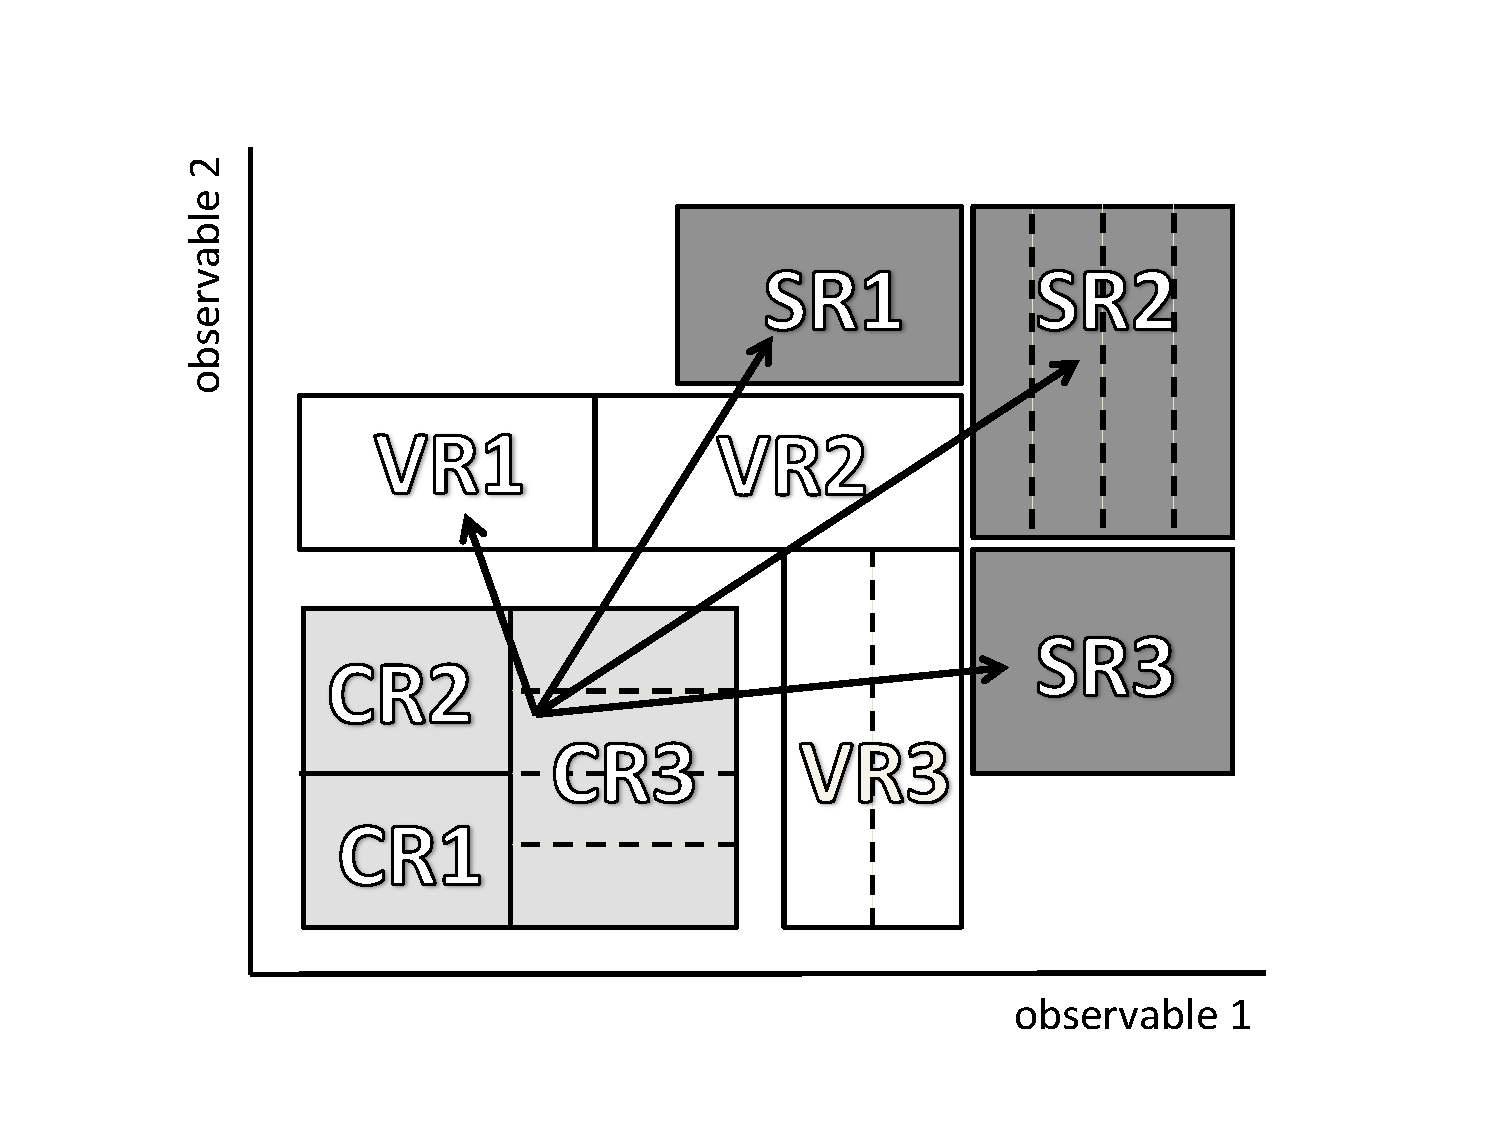
\includegraphics[scale=0.4]{cartoon_CRVRSR_bw.pdf}
        \caption{A illustration of multiple signal, control, and validation regions.
        The background contamination in the SRs can be estimated by extrapolating from the CRs and is verified in the VRs which lie in between the SRs and CRs.
        All regions can be single bin or multiple bins which are indicated by the dashed lines.
        The figure is taken from~\cite{Baak:2014wma}.}
        \label{fig:bkg_SRs_CRs_VRs}
    \end{center}
\end{figure}

%%%
%%%
%%%

\subsection{Specific to this analysis}
\label{subsec:bkg_SRs_CRs_VRs_spicific}
Table~\ref{tab:bkg_background_processes} lists the SM background processes for this analysis, the origins in the SR, and the estimation strategies.
In order to estimate and validate the background contaminations in SR, two CRs and three VRs are defined.
Table~\ref{tab:bkg_CRs_VRs_definitions} lists the definitions of CRs and VRs where the common selection criteria listed in Table~\ref{tab:event_signal_region} have been applied.
The CR-top is used to estimate the \ttbar and $tW$ contaminations in SR.
The CR-tau is used to estimate the  $Z^{(*)}/\gamma^{*}(\to \tau \tau)$+jets contamination in SR.
The VR-VV is used for validating diboson background, the VR-SS is used for validating same-sign dilepton background, and VRDF-$m_{\ell \ell}$ is used for validating the background come from different flavor leptons, which include both $e \mu$ and $\mu e$.

\begin{table}[htbp]
    %\begin{center}
    \resizebox{\textwidth}{!}{% <------ Don't forget this %
        \begin{tabular}{lll}
            \hline
            \hline
            Background process                             & Origin in SR                                             & Estimation strategy\\
            \hline
            \ttbar, $tW$ ($\to 2\ell$)                     & irreducible, $b$-jet fails identification                & CR using $b$-tagging\\
            $Z^{(*)}/\gamma^{*}(\to \tau \tau)$+jets       & irreducible fully leptonic $\tau$                        & CR using $m_{\tau \tau}$\\
            $Z^{(*)}/\gamma^{*}(\to ee, \mu \mu)$+jets     & instrumental \met                                        & MC\\
            loss mass Drell-Yen                            & instrumental \met                                        & MC, data-driven cross check\\
            fakes ($W$+jets, $VV(1\ell)$, \ttbar($1\ell$)) & jet fakes $2^\mathrm{nd}$ lepton                         & fake factor, SS VR\\
            $VV$                                           & irreducible dileptonic and missed $3^\mathrm{rd}$ lepton & MC, VR using $\met/H_\mathrm{T}^\mathrm{leptons}$\\
            other rare processes                          & irreducible leptonic decays                              & MC\\
            \hline
            \hline
        \end{tabular}
    }
    %\end{center}
    \caption{The background processes for the 2$\ell$ analysis and the strategy for estimating the background contamination in the SR.}
    \label{tab:bkg_background_processes}
\end{table}

\begin{table}[htbp]
    %\begin{center}
    \resizebox{\textwidth}{!}{% <------ Don't forget this %
        %{\scriptsize
            \begin{tabular}{llll}
                \hline
                \hline
                Region               & Leptons                                                                        & $\met/H_{\mathrm{T}}^{\mathrm{lep}}$                & Additional requirements\\
                \hline
                CR-top               & $e^{\pm}e^{\mp}$, $\mu^{\pm}\mu^{\mp}$, $e^{\pm}\mu^{\mp}$, $\mu^{\pm}e^{\mp}$ & $> 5$                                               & $\ge 1 b$-tagged jet(s)\\
                CR-tau               & $e^{\pm}e^{\mp}$, $\mu^{\pm}\mu^{\mp}$, $e^{\pm}\mu^{\mp}$, $\mu^{\pm}e^{\mp}$ & $\in$ [4, 8]                                        & $m_{\tau \tau} \in$ [60, 120]~{\GeV}\\
                \hline
                VR-VV                & $e^{\pm}e^{\mp}$, $\mu^{\pm}\mu^{\mp}$, $e^{\pm}\mu^{\mp}$, $\mu^{\pm}e^{\mp}$ & $< 3$                                               & -\\
                VR-SS                & $e^{\pm}e^{\pm}$, $\mu^{\pm}\mu^{\pm}$, $e^{\pm}\mu^{\pm}$, $\mu^{\pm}e^{\pm}$ & $> 5$                                               & -\\
                VRDF-$m_{\ell \ell}$ & $e^{\pm}\mu^{\mp}$, $\mu^{\pm}e^{\mp}$                                         & $>$ max(5, 15 - 2 $m_{\ell \ell}/1~{\GeV}$)         & $\Delta R_{\ell \ell} < 2$, $m_{\mathrm{T}}^{\ell_{1}} < 70$~{\GeV}\\
                \hline
                \hline
            \end{tabular}
        %}
    }
    %\end{center}
    \caption{Definition of control regions and validation regions.}
    \label{tab:bkg_CRs_VRs_definitions}
\end{table}%

%%%
%%%
%%%

\section{Irreducible background}
\label{sec:bkg_irreducible_background}
The irreducible background for this analysis are the SM processes containing two prompt leptons, \met, and jets.
Therefor, they can enter the SR and mimic the signal events.
The dominant sources are the \ttbar, $tW$, and $Z^{(*)}/\gamma^{*}(\to \tau \tau)$+jets processes.
These processes decay to same flavor lepton pairs ($ee$ and $\mu \mu$) and different flavor lepton pairs ($e \mu$ and $\mu e$) at the same rates.
When defining the CR-top and CR-tau, all possible flavor $e^{\pm} e^{\mp}$, $\mu^{\pm} \mu^{\mp}$, $e^{\pm} \mu^{\pm}$, $\mu^{\pm} e^{\mp}$ are consider to enhance the statistics.
By requiring the events with at least one $b$-tagged jet, the CR-top defined a top quarks enriched region with $\sim$72\% purity.
The CR-top is used to estimate the \ttbar and $tW$ decaying to 2$\ell$ final states in the SR.
By requiring the events satisfying $60 < m_{\tau \tau} < 120$~{\GeV} and $\met/H_{\mathrm{T}}^{\mathrm{lep}}$ between 4 and 8 to reduce the signal contaminations, the CR-tau defined a $Z^{(*)}/\gamma^{*}(\to \tau \tau)$+jets enriched region with $\sim$80\% purity.
The CR-tau is used to estimate the leptonic $\tau$ contaminations in the SR.
The kinematic distributions of $\met/H_\mathrm{T}^\mathrm{lep}$ and $m_{\tau \tau}$ in the CR-top and CR-tau after performing background-only fit are shown in Fig~\ref{fig:bkg_kinematic_distributions_in_CRs}.
All the event selection criteria are applied except the variable being plotted.
The expected background contributions from different processes are stacked and compared with the data.

\begin{figure}[ht]
    \begin{center}
        \begin{subfigure}[b]{0.48\textwidth}
            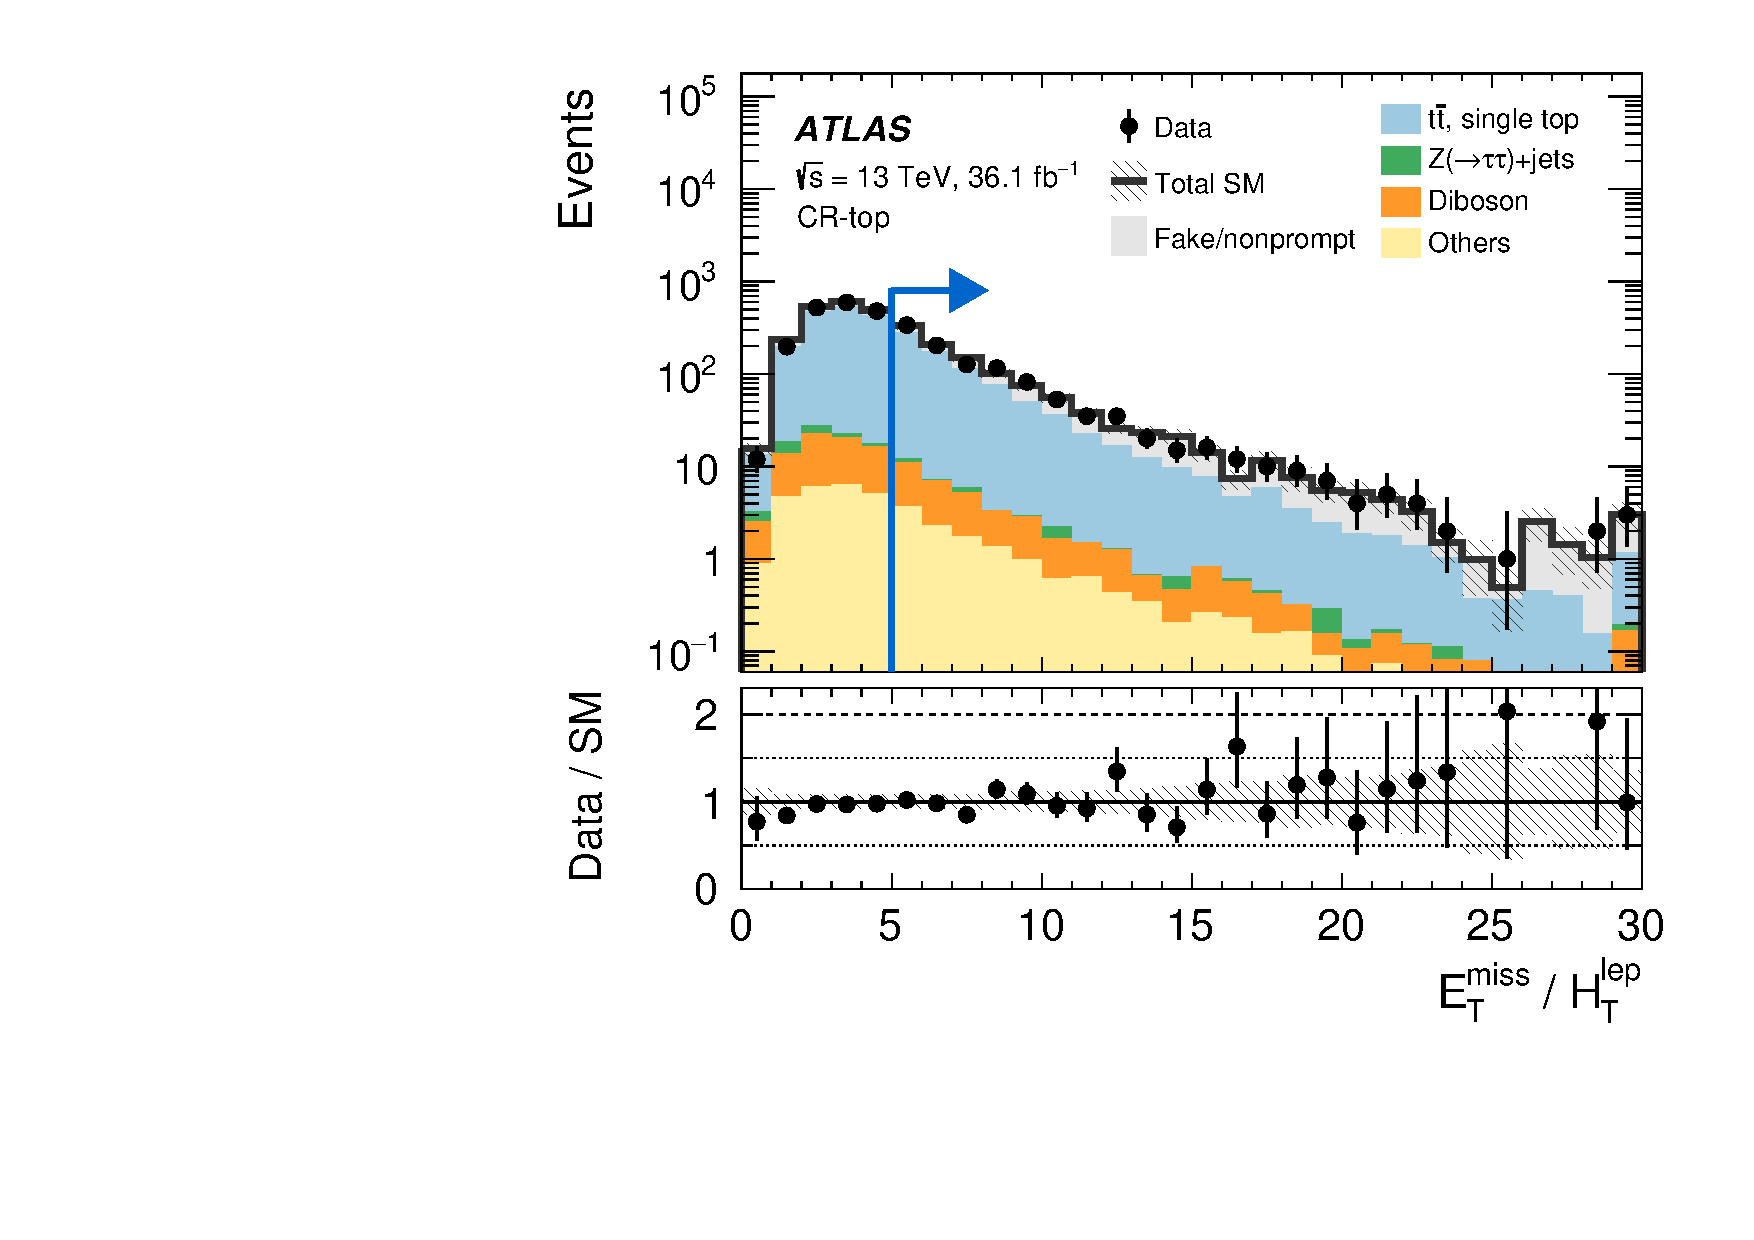
\includegraphics[scale=0.35]{Higgsino_bkg_CRtop_CRtop_METOverHTLep_METOverHTLep.pdf}
            \caption{{\footnotesize The $\met/H_\mathrm{T}^\mathrm{lep}$ distribution in CR-top.}}
            \label{fig:bkg_kinematic_metOverHT_CRtop}
        \end{subfigure}
        \begin{subfigure}[b]{0.48\textwidth}
            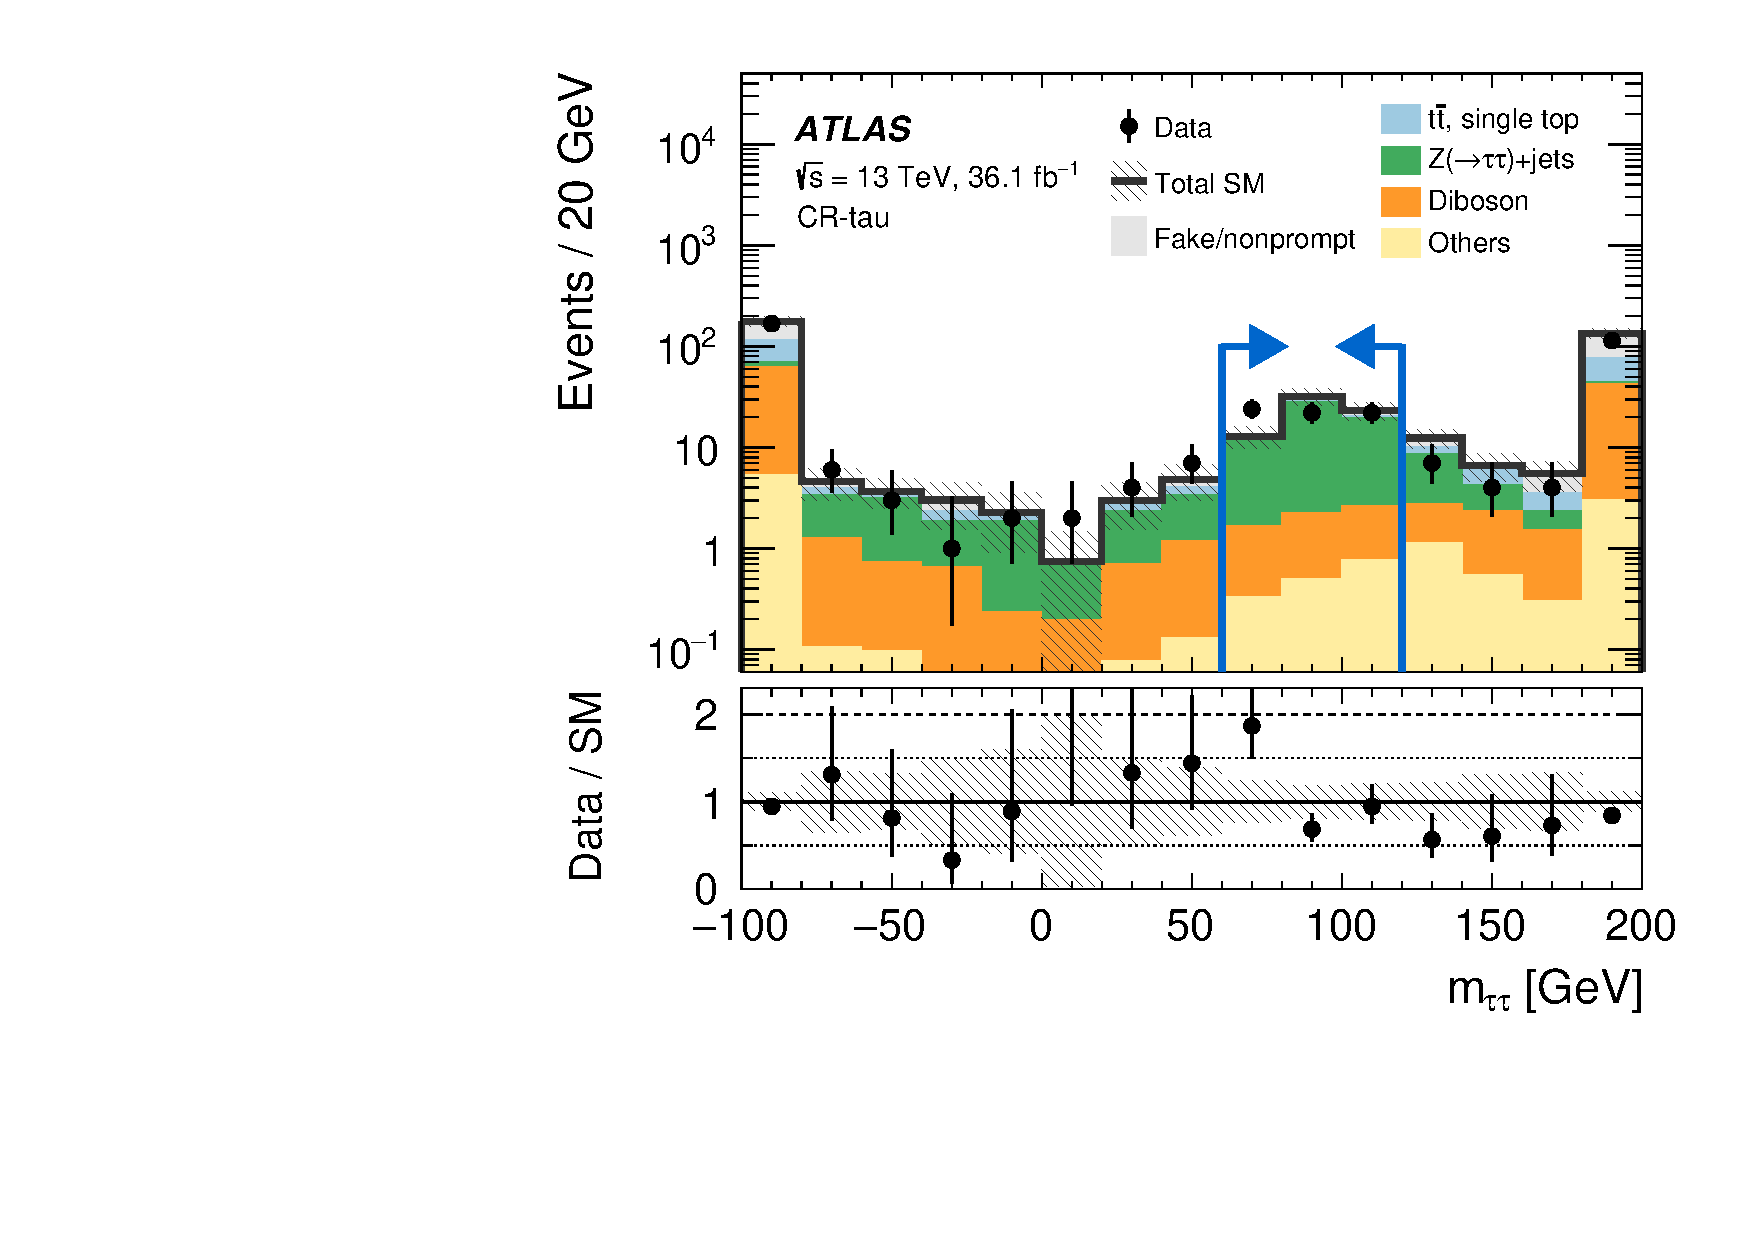
\includegraphics[scale=0.35]{Higgsino_bkg_CRtau_CRtau_MTauTau_MTauTau.pdf}
            \caption{The $m_{\tau \tau}$ distribution in CR-tau.}
            \label{fig:bkg_kinematic_mtautau_CRtau}
        \end{subfigure}
        \caption{The kinematic distributions of $\met/H_\mathrm{T}^\mathrm{lep}$ and $m_{\tau \tau}$ in the CR-top and CR-tau, respectively.
        All the event selection criteria are applied except the variable being plotted and the background-only fits are performed.
        The selection requirement of the plotting variable is indicated by the blue arrows.
        The first and last bins include the underflow and overflow, respectively.
        The expected background contributions from different processes are stacked and compared with the data.}
        \label{fig:bkg_kinematic_distributions_in_CRs}
    \end{center}
\end{figure}

The diboson $VV$ events and the rare processes are also contributed to the irreducible background.
But it is difficult to have pure diboson or rare sample that can be used to estimate the contaminations in SR.
Therefore, the background contaminations are estimated using MC simulation and validated by the VR-VV.
By requiring $\met/H_\mathrm{T}^\mathrm{lep} < 3$, the signal contamination in the VR-VV is at most 8\% in the samples, the diboson events contribute $\sim$40\%, fake lepton events contribute $\sim$25\%, \ttbar and single top events contribute $\sim$23\%, and the rest parts are smaller and contributed by the other processes.

The VRDF-$m_{\ell \ell}$ validation region is constructed using different flavor ($e\mu$ and $\mu e$) leptons.
This VR has the same selection criteria as the SR, except the leptons are composed by different flavor.
Since the irreducible background are symmetric in $ee+\mu\mu$ and $e\mu+\mu e$, the VRDF-$m_{\ell \ell}$ is used to check the eventual extrapolation in the fitting procedure within the same kinematic as SR.
The signal contamination in this VR is less than 8\%.

%%%
%%%
%%%

\section{Reducible background}
\label{sec:bkg_reducible_background}
The main contributions of the reducible background come from the non-prompt leptons and the processes that the reconstructed \met are instrumental in origin.

%%%
%%%
%%%

\subsection{Fake/non-prompt lepton background}
\label{subsec:bkg_fake_lepton_background}
The background of non-prompt leptons, or called fake leptons, mainly come from the $W$+jets, VV, \ttbar processes.
In these processes, a jet is misidentified as a lepton and form a dilepton final state in the SR.
Because the MC simulation couldn't model fake leptons well, a data-driven Fake Factor method~\cite{ATLAS:2014aga} is used to estimate the fake lepton contamination in the SR. 

%%%
%%%
%%%

\subsubsection{Fake factor method}
\label{subsubsec:bkg_fake_factor_method}
The Fake Factor method defined a tight set and a loose set of lepton identification criteria.
The tight set refers as ID and the loose set refers as anti-ID.
The ID leptons correspond to the requirements applied to signal leptons used in the analysis.
The anti-ID leptons define a fake leptons enriched sample by releasing or inverting one or more of the identification, isolation, or impact parameter $|d_{0}|/\sigma(d_{0})$ requirements relative to the signal leptons.
Therefore, the leptons in ID and anti-ID are orthogonal.
Then the fake factor $F$ is defined as the ratio between the number of ID and the number of anti-ID leptons as shown in Eq.~\ref{eq:bkg_fake_factor}.

\begin{equation}
    F = \frac{N_\mathrm{ID}}{N_\mathrm{anti-ID}}
    \label{eq:bkg_fake_factor}
\end{equation}

The $N_\mathrm{anti-ID}$ is the number of fake leptons in the anti-ID measurement region where the contributions from prompt leptons are subtracted using the MC simulation results.
The $F$ for electron and muon are measured in a fake leptons enriched region as a function of reconstructed lepton \pt and are used to estimate the reducible background in the SR.
These $F$ are applied to events in anti-ID control region, which has the same selection criteria as SR, except an ID lepton is replaced by an anti-ID lepton.
The total reducible background in the SR can be estimated by

\begin{equation}
    N^\mathrm{SR}_\mathrm{est} = F \cdot N^\mathrm{CR}_\mathrm{fake}
    \label{eq:bkg_estimated_fake_leptons}
\end{equation}

The schematic illustration of the fake factor method is shown in Fig.~\ref{fig:bkg_fake_factor_method}.

\begin{figure}[htb]
    \begin{center}
        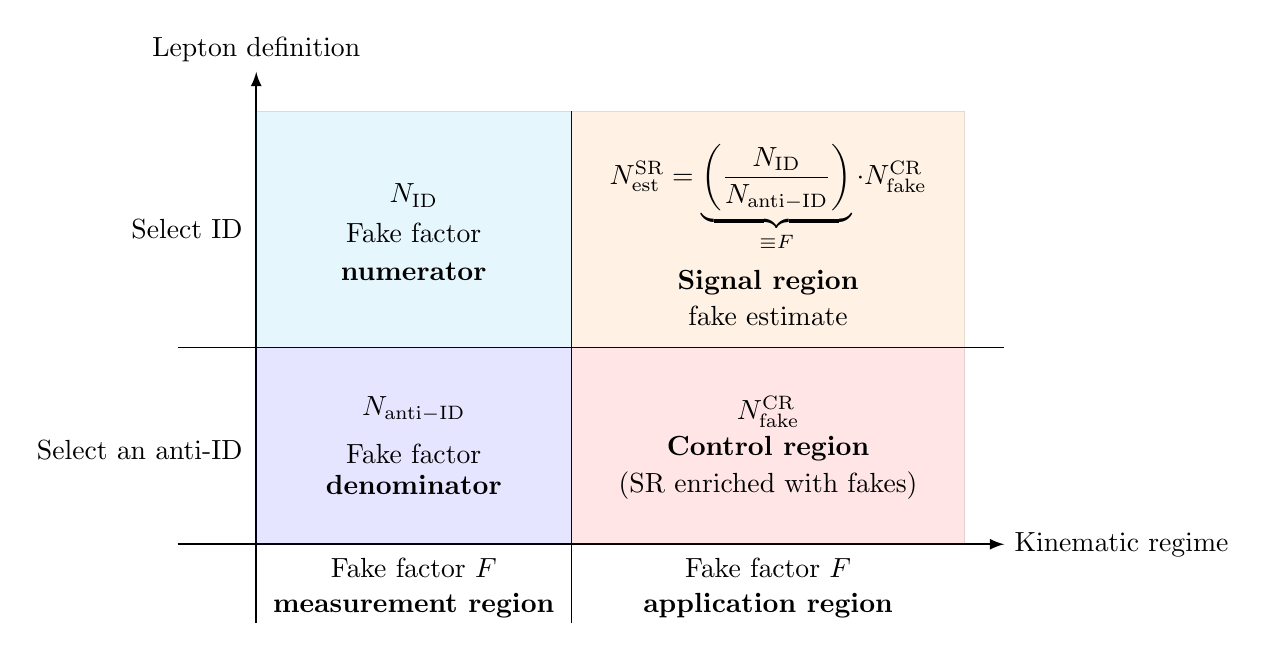
\begin{tikzpicture}
    
    % axes
    \draw [-latex, thick] (-1,0)--(9.5,0) node [right] {Kinematic regime};
    \draw [-latex, thick] (0,-1)--(0,6) node [above] {Lepton definition};
    
    % selection 
    \draw (4,-1) -- (4,5.5);
    \draw (-1,2.5) -- (9.5,2.5);
    
    % axis labels
    \node at (-0.05,4) [left] {Select ID};
    \node at (-0.05,1.2) [left] {Select an anti-ID};
    
    \node at (2,-0.05) [below] {Fake factor $F$};
    \node at (2,-0.5) [below] {\textbf{measurement region}};
    \node at (6.5,-0.05) [below] {Fake factor $F$};
    \node at (6.5,-0.5) [below] {\textbf{application region}};
    
    % boxes
    \draw [opacity=0.1, fill=blue] (0,0) -- (0,2.5)-- (4,2.5) -- (4,0) -- (0,0);
    \draw [opacity=0.1, fill=cyan] (0,2.5) -- (0,5.5)-- (4,5.5) -- (4,2.5) -- (0,2.5);
    \draw [opacity=0.1, fill=red] (4,0) -- (4,2.5)-- (9,2.5) -- (9,0) -- (4,0);
    \draw [opacity=0.1, fill=orange] (4,2.5) -- (4,5.5)-- (9,5.5) -- (9,2.5) -- (4,2.5);
    
    % box labels
    \node at (2,2) [below] {$N_\mathrm{anti-ID}$};
    \node at (2,1.4) [below] {Fake factor};
    \node at (2,1) [below] {\textbf{denominator}};
    
    \node at (2,4.7) [below] {$N_\mathrm{ID}$};
    \node at (2,4.2) [below] {Fake factor};
    \node at (2,3.7) [below] {\textbf{numerator}};
    
    \node at (6.5,5.2) [below] {$N^\mathrm{SR}_\mathrm{est} = \underbrace{\left(\displaystyle\frac{N_\mathrm{ID}}{N_\mathrm{anti-ID}}\right)}_{\equiv F}\cdot N^\mathrm{CR}_\mathrm{fake}$};
    \node at (6.5,3.6) [below] {\textbf{Signal region}};
    \node at (6.5,3.15) [below] {fake estimate};
    
    \node at (6.5,2) [below] {$N^\mathrm{CR}_\mathrm{fake}$};
    \node at (6.5,1.5) [below] {\textbf{Control region}};
    \node at (6.5,1.05) [below] {(SR enriched with fakes)};
    
\end{tikzpicture}

        \caption{The schematic illustration of the fake factor method used to estimate the fake lepton contribution in the SR.}
        \label{fig:bkg_fake_factor_method}
    \end{center}
\end{figure}

%%%
%%%
%%%

\subsubsection{Specific to this analysis}
\label{subsubsec:bkg_fake_specific}
The ID electrons are the signal electrons as shown in Table~\ref{tab:event_object_definitions} and the anti-ID electrons are baseline electrons passing \texttt{LooseAndBLayer} identification but failing at least one of the following requirements: \texttt{Tight} identification, \texttt{GradientLoose} isolation, or $|d_{0}/\sigma(d_{0})| < 5$.
The ID muons are the signal muons as shown in Table~\ref{tab:event_object_definitions} and the anti-ID muons are baseline muons failing either \texttt{FixedCutTightTrackOnly} isolation or $|d_{0}/\sigma(d_{0})| < 3$.
Both ID and anti-ID leptons are required to satisfy $|z_{0} \sin \theta| < 0.5$~mm to reduce the impact of pileup.
Table~\ref{tab:bkg_ID_anti_ID_selection_criteria} summarizes the ID and anti-ID selection criteria for electrons and muons.

\begin{table}[htbp]
    %\begin{center}
    \resizebox{\textwidth}{!}{% <------ Don't forget this %
        {\footnotesize
            \begin{tabular}{lll}
                \hline
                \hline
                                 & Electrons                           & Muons\\
                \hline
                Kinematic        & $\pt > 4.5$~{\GeV}, $|\eta| < 2.47$ & $\pt > 4$~{\GeV}, $|\eta| < 2.5$\\
                Identification   & pass \texttt{LooseAndBLayerLLH}     & pass \texttt{Medium}\\
                Impact parameter & $|z_{0} \sin \theta| < 0.5$~mm      & $|z_{0} \sin \theta| < 0.5$~mm\\
                \hline
                \multicolumn{3}{c}{anti-ID have to fail at least one of the requirements}\\
                \hline
                Identification   & \texttt{TightLLH}                   & -\\
                Isolation        & \texttt{GradientLooseLLH}           & \texttt{FixedCutTightTrackOnlyLLH}\\
                Impact parameter & $|d_{0}/\sigma(d_{0})| < 5$         & $|d_{0}/\sigma(d_{0})| < 3$\\
                \hline
                \hline
            \end{tabular}
        }
    }
    %\end{center}
    \caption{The ID and anti-ID selection criteria for electrons and muons.}
    \label{tab:bkg_ID_anti_ID_selection_criteria}
\end{table}

The electrons and muons fake factor depend on the lepton \pt largely and on the leading jet \pt.
Therefore, the leading jet \pt for the events used for fake factor measurement are required to be greater than 100~{\GeV} making the fake factor measurement region similar to SR.
The muon fake factor also depends on the $N_{b-\mathrm{jet}}$ in the events, the estimated number of fake lepton in CR-top is calculated using events with at least one $b$-jet while the estimated number of fake lepton in the other regions are computed using zero $b$-jet events.
The electrons and muons fake factor are computed using events with $m_\mathrm{T} < 40$~{\GeV} in different \pt bins.
Figure~\ref{fig:bkg_electron_fake_factor} shows the electrons fake factors as a function of \pt and leading jet \pt and Fig~\ref{fig:bkg_muon_fake_factor} shows the muons fake factor as a function of \pt with 0 $b$-jet and at least one $b$-jet.

\begin{figure}[ht]
    \begin{center}
        \begin{subfigure}[b]{0.48\textwidth}
            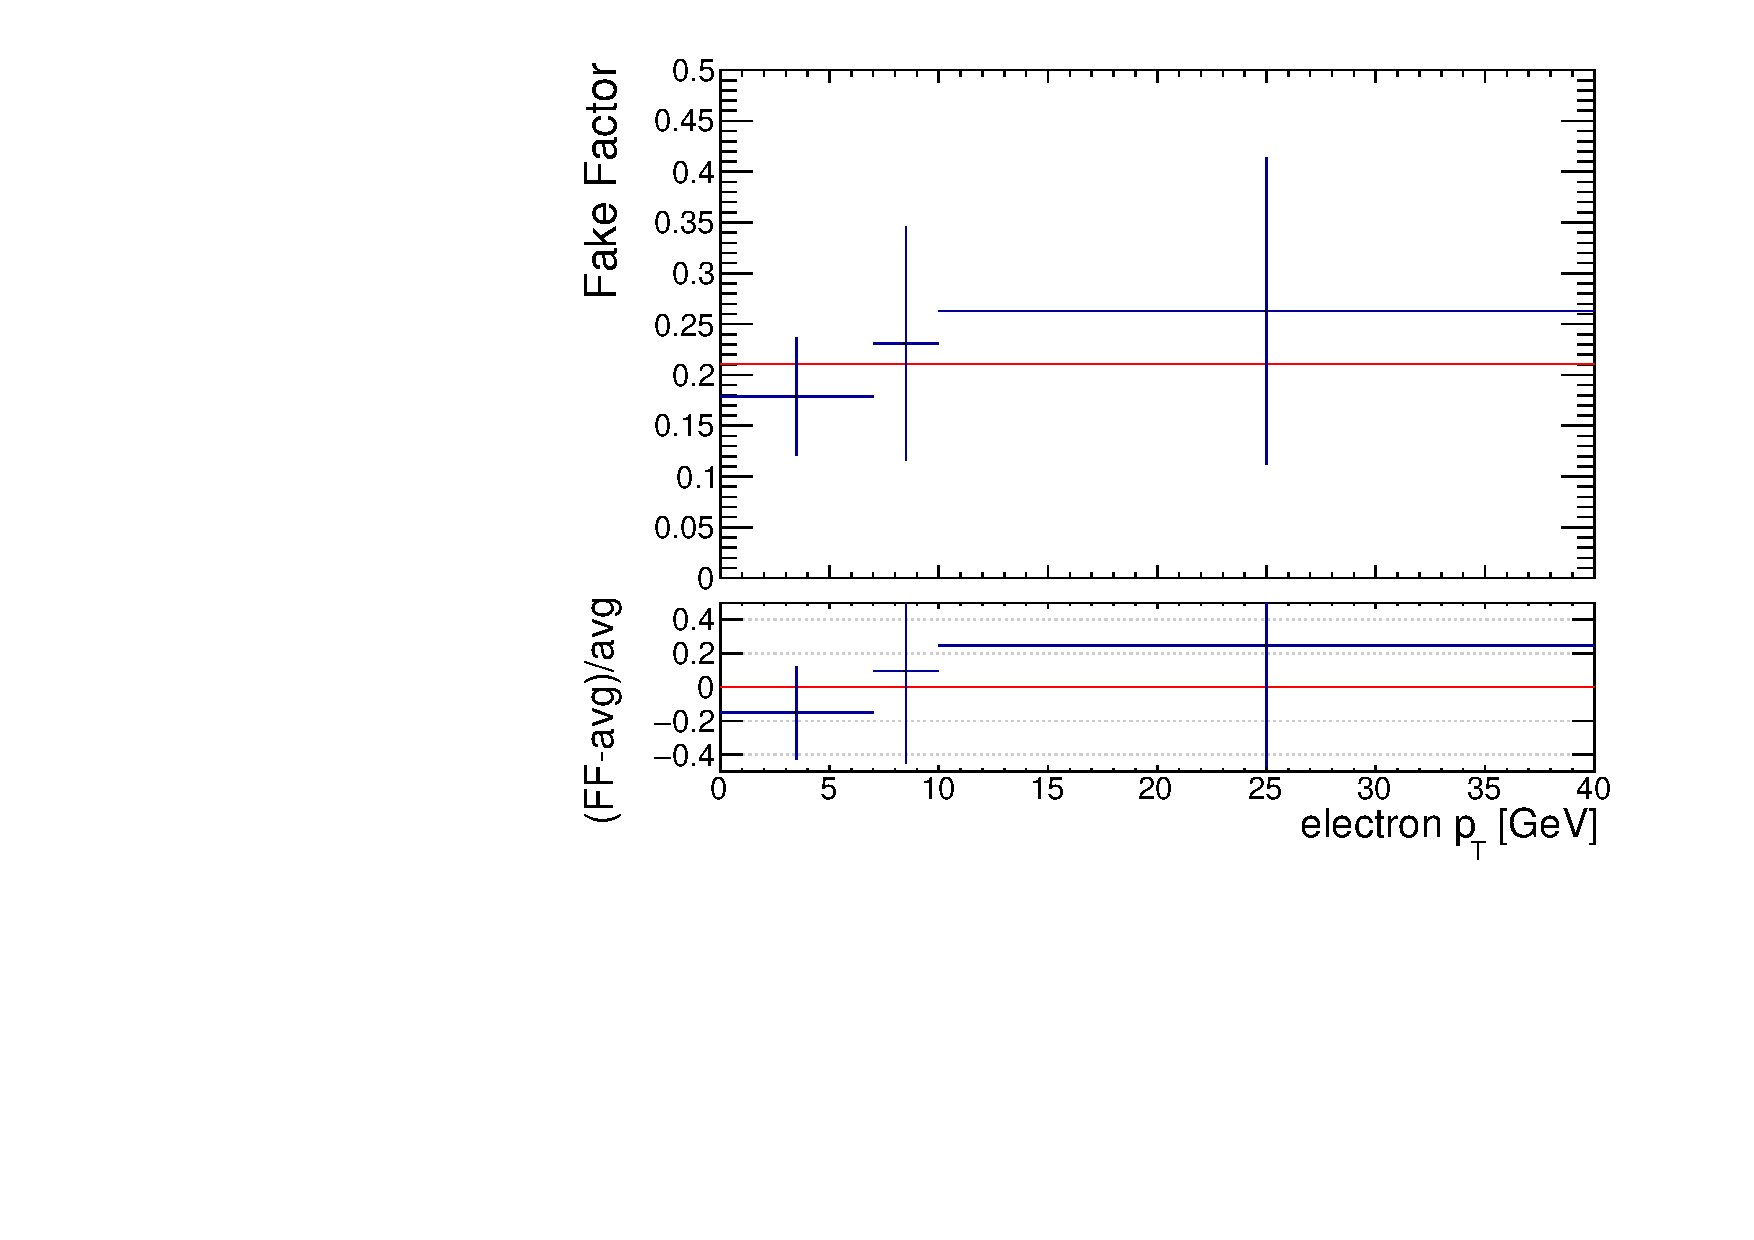
\includegraphics[scale=0.35]{FakeFactor_el_pt.pdf}
            \caption{Electron \pt dependence}
            \label{fig:bkg_electron_fake_factor_pt}
        \end{subfigure}
        \begin{subfigure}[b]{0.48\textwidth}
            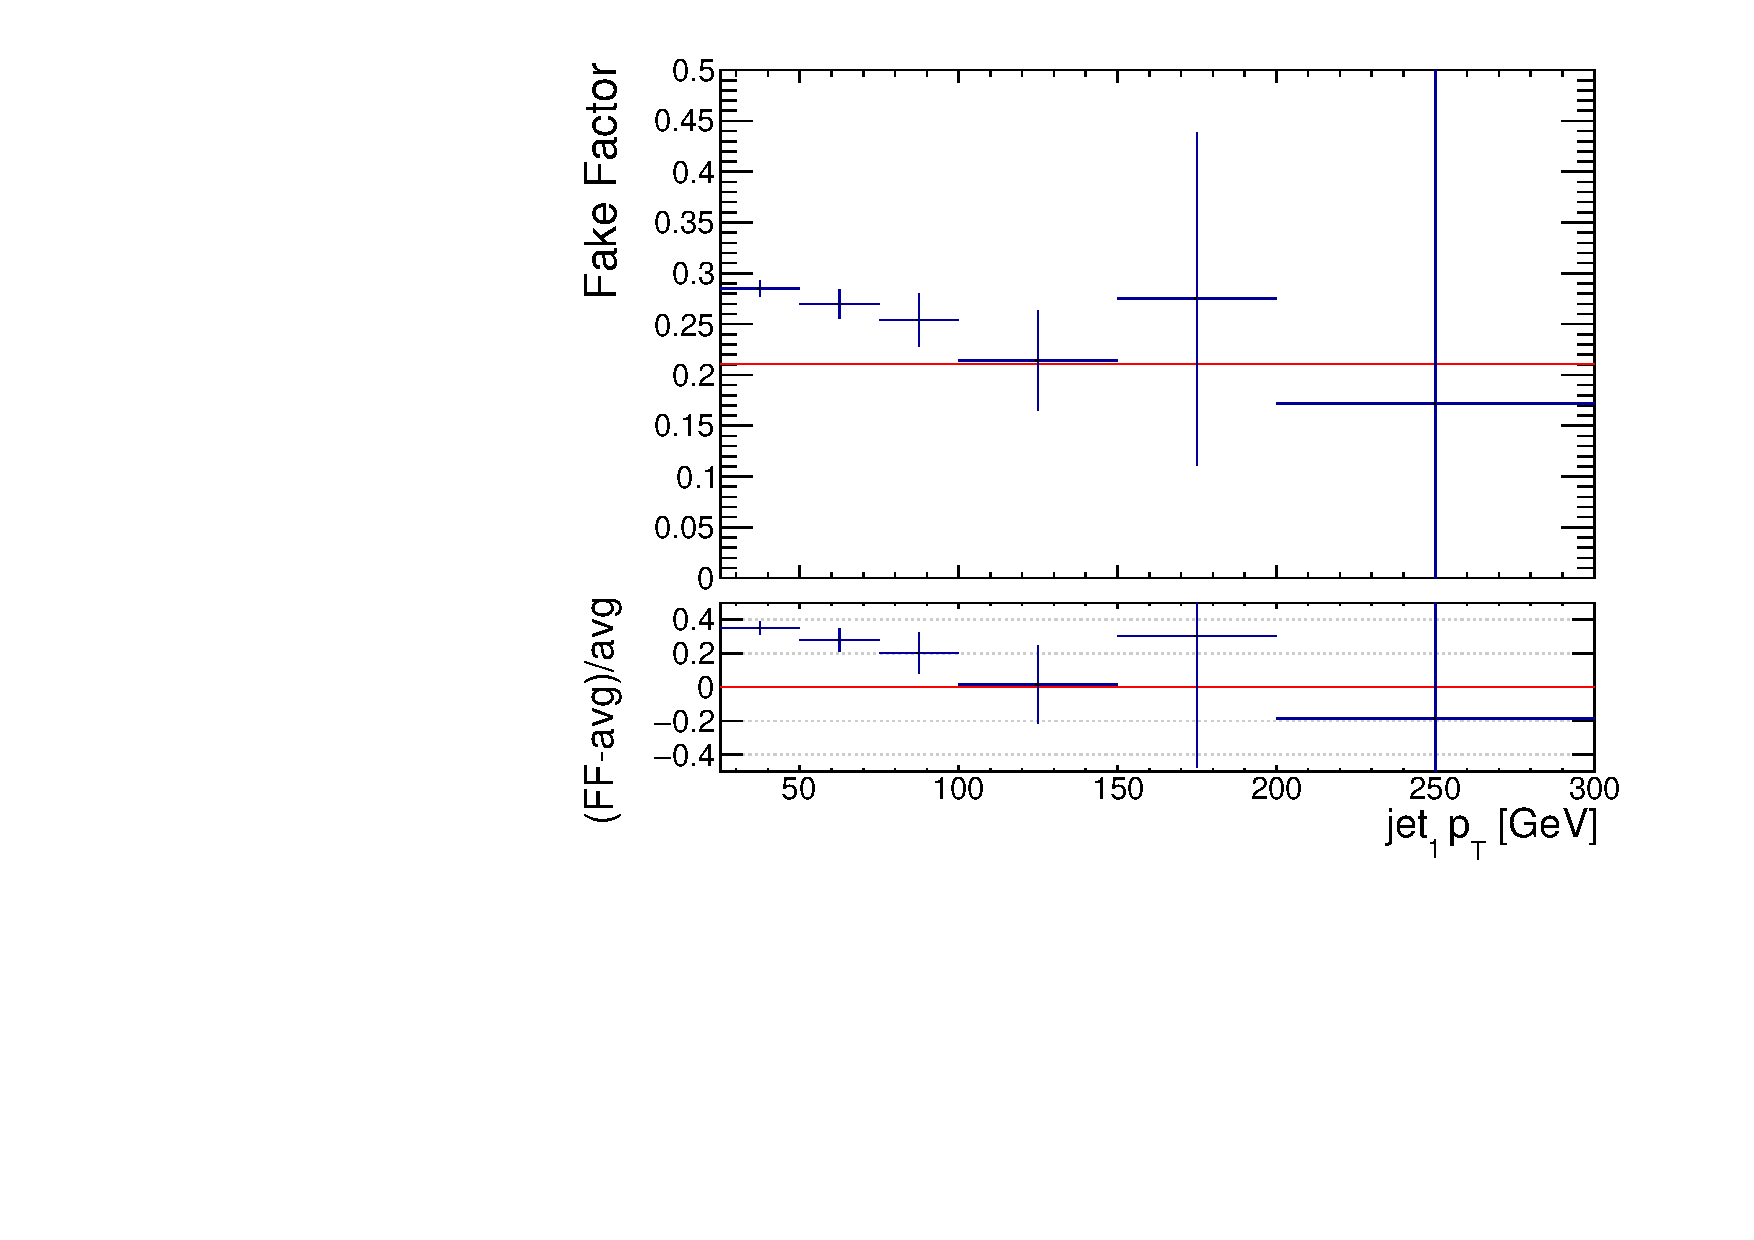
\includegraphics[scale=0.35]{FakeFactor_el_j1pt.pdf}
            \caption{Leading jet \pt dependence}
            \label{fig:bkg_electron_fake_factor_leading_jet_pt}
        \end{subfigure}
        \caption{The electron fake factor as a function of \pt and leading jet \pt.
        The red line is the average electron fake factor.}
        \label{fig:bkg_electron_fake_factor}
    \end{center}
\end{figure}

\begin{figure}[ht]
    \begin{center}
        \begin{subfigure}[b]{0.48\textwidth}
            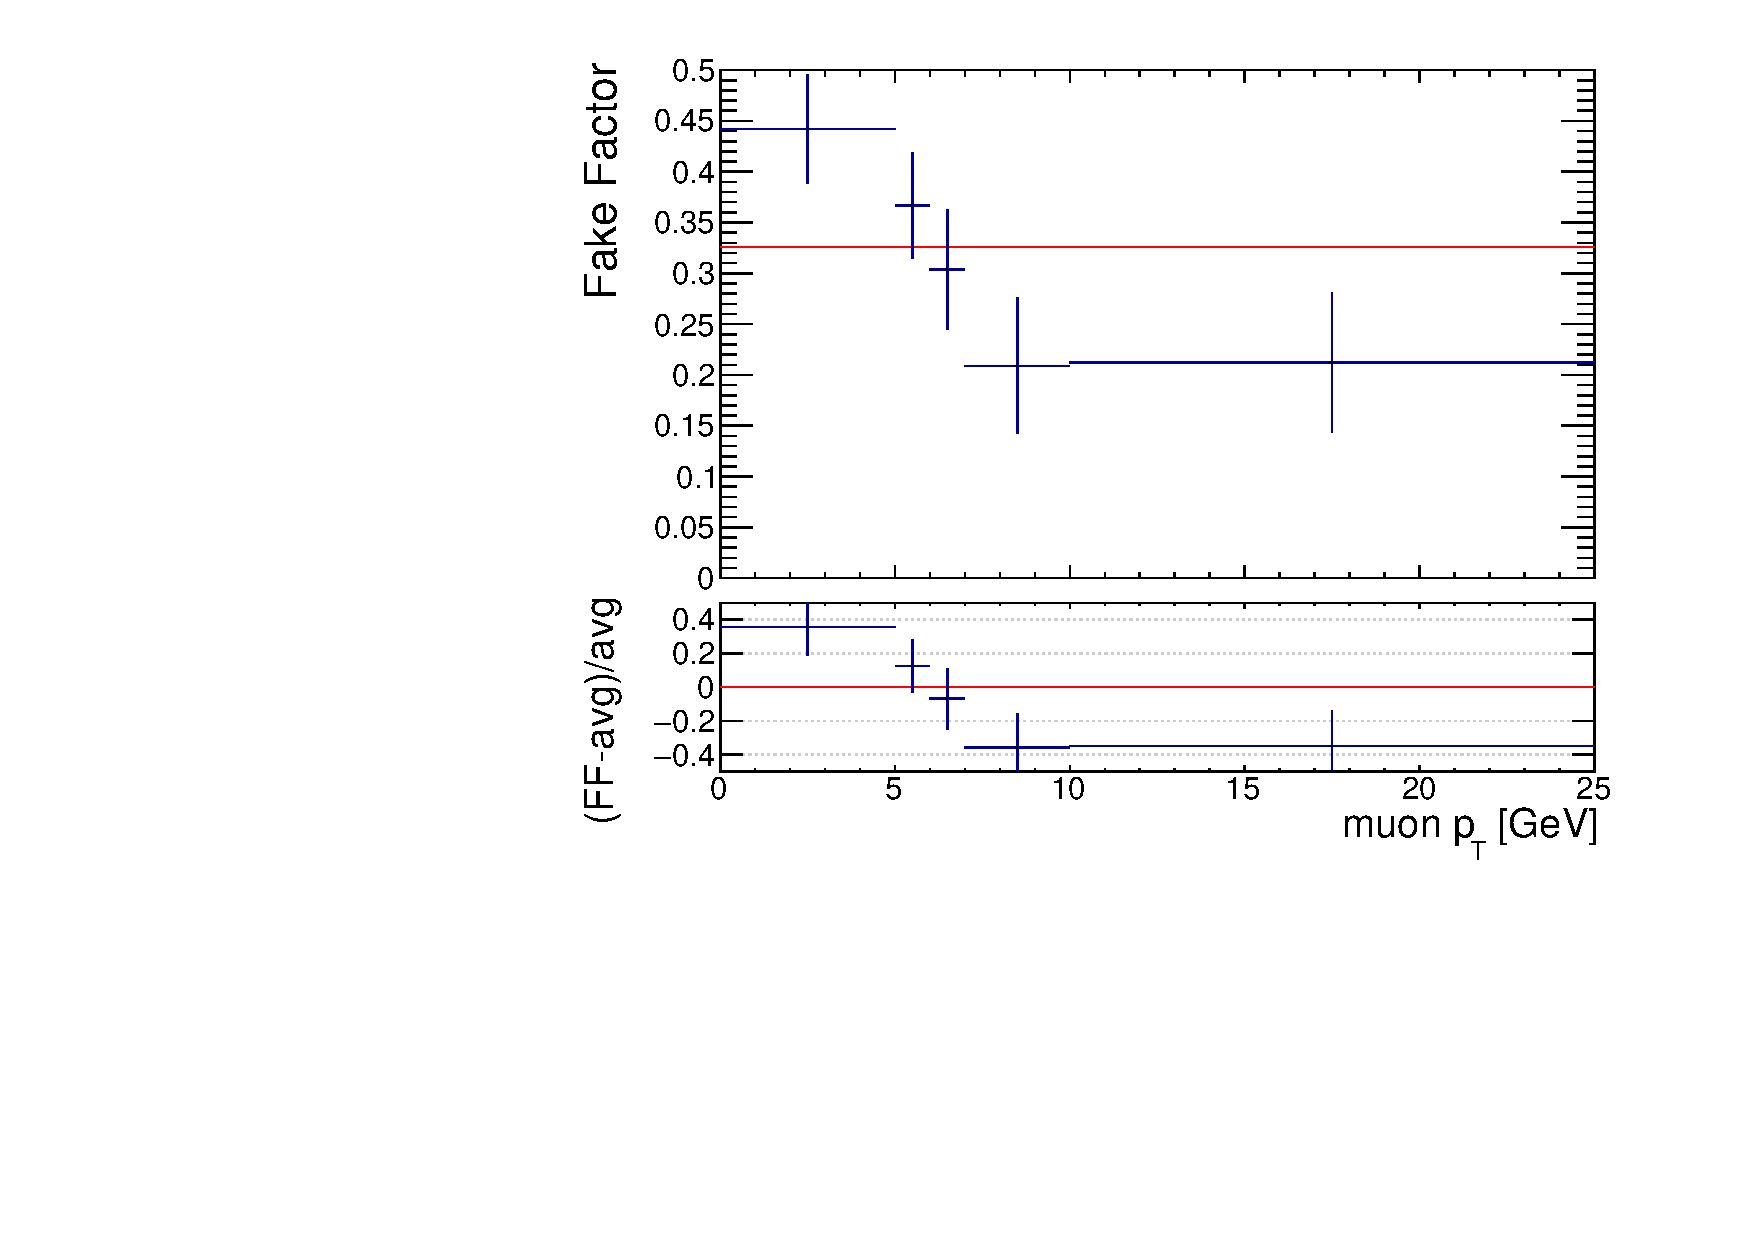
\includegraphics[scale=0.35]{FakeFactor_mu_ptb0.pdf}
            \caption{Muon \pt dependence with 0 $b$-jet}
            \label{fig:bkg_muon_fake_factor_pt_0bjet}
        \end{subfigure}
        \begin{subfigure}[b]{0.48\textwidth}
            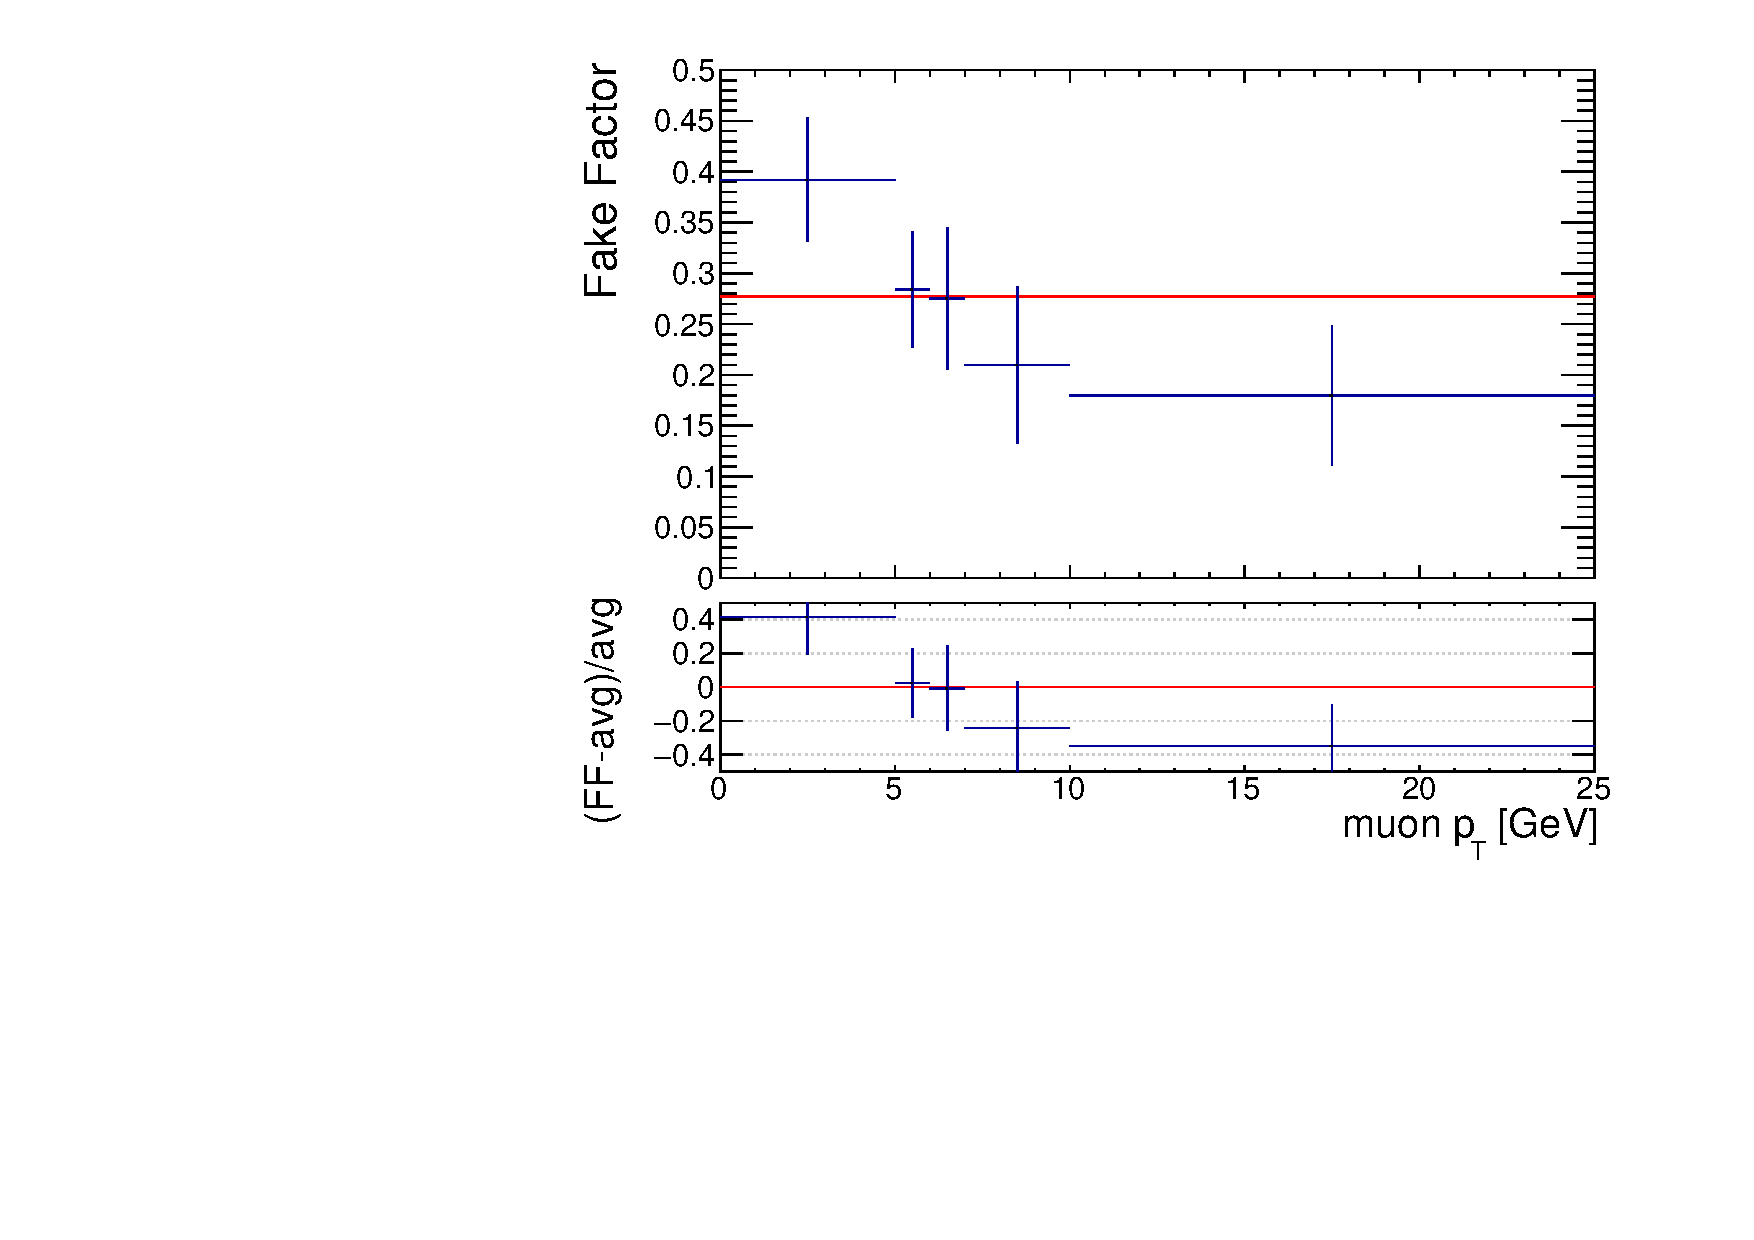
\includegraphics[scale=0.35]{FakeFactor_mu_ptb1.pdf}
            \caption{Muon \pt dependence with $\ge 1 b$-jet}
            \label{fig:bkg_muon_fake_factor_pt_bjets}
        \end{subfigure}
        \caption{The muon fake factor as a function of \pt with 0 $b$-jet and at least one $b$-jet.
        The red line is the average muon fake factor.}
        \label{fig:bkg_muon_fake_factor}
    \end{center}
\end{figure}

%%%
%%%
%%%

\subsection{Instrumental \met background}
\label{subsec:bkg_instrumental_met_background}
The detector mismeasuring leptons or jets in the background processes which don't contain invisible particle might satisfy the $\met > 200$~{\GeV} requirement.
For example, the $Z^{(*)}/\gamma^{*}(\to ee, \mu \mu)$+jets Drell-Yan dilepton production can enter the SR due to the instrumental \met.
By requiring $\met > 200$~{\GeV}, the contributions from these background processes are expected very small.
Using the MC simulation, these process are found to be negligible.
The small mass splitting between $\widetilde{\chi}^{0}_{2}$ and $\widetilde{\chi}^{0}_{1}$ causes the low invariant dilepton mass where the dilepton events are the decay product of $\widetilde{\chi}^{0}_{2}$.
The $e^{\pm} e^{\mp}$ and $\mu^{\pm} \mu^{\mp}$ invariant masses for data events passing \met trigger and $|\Delta \phi(j_{1}, \mathbf{p}_\mathrm{T}^\mathrm{miss})| < 1.5$ are shown in Fig.~\ref{fig:bkg_invariant_mass} where a $J/\psi$ peak $3.0 < m_{\ell \ell} < 3.2$~{\GeV} can be seen.

\begin{figure}[ht]
    \begin{center}
        \begin{subfigure}[b]{0.48\textwidth}
            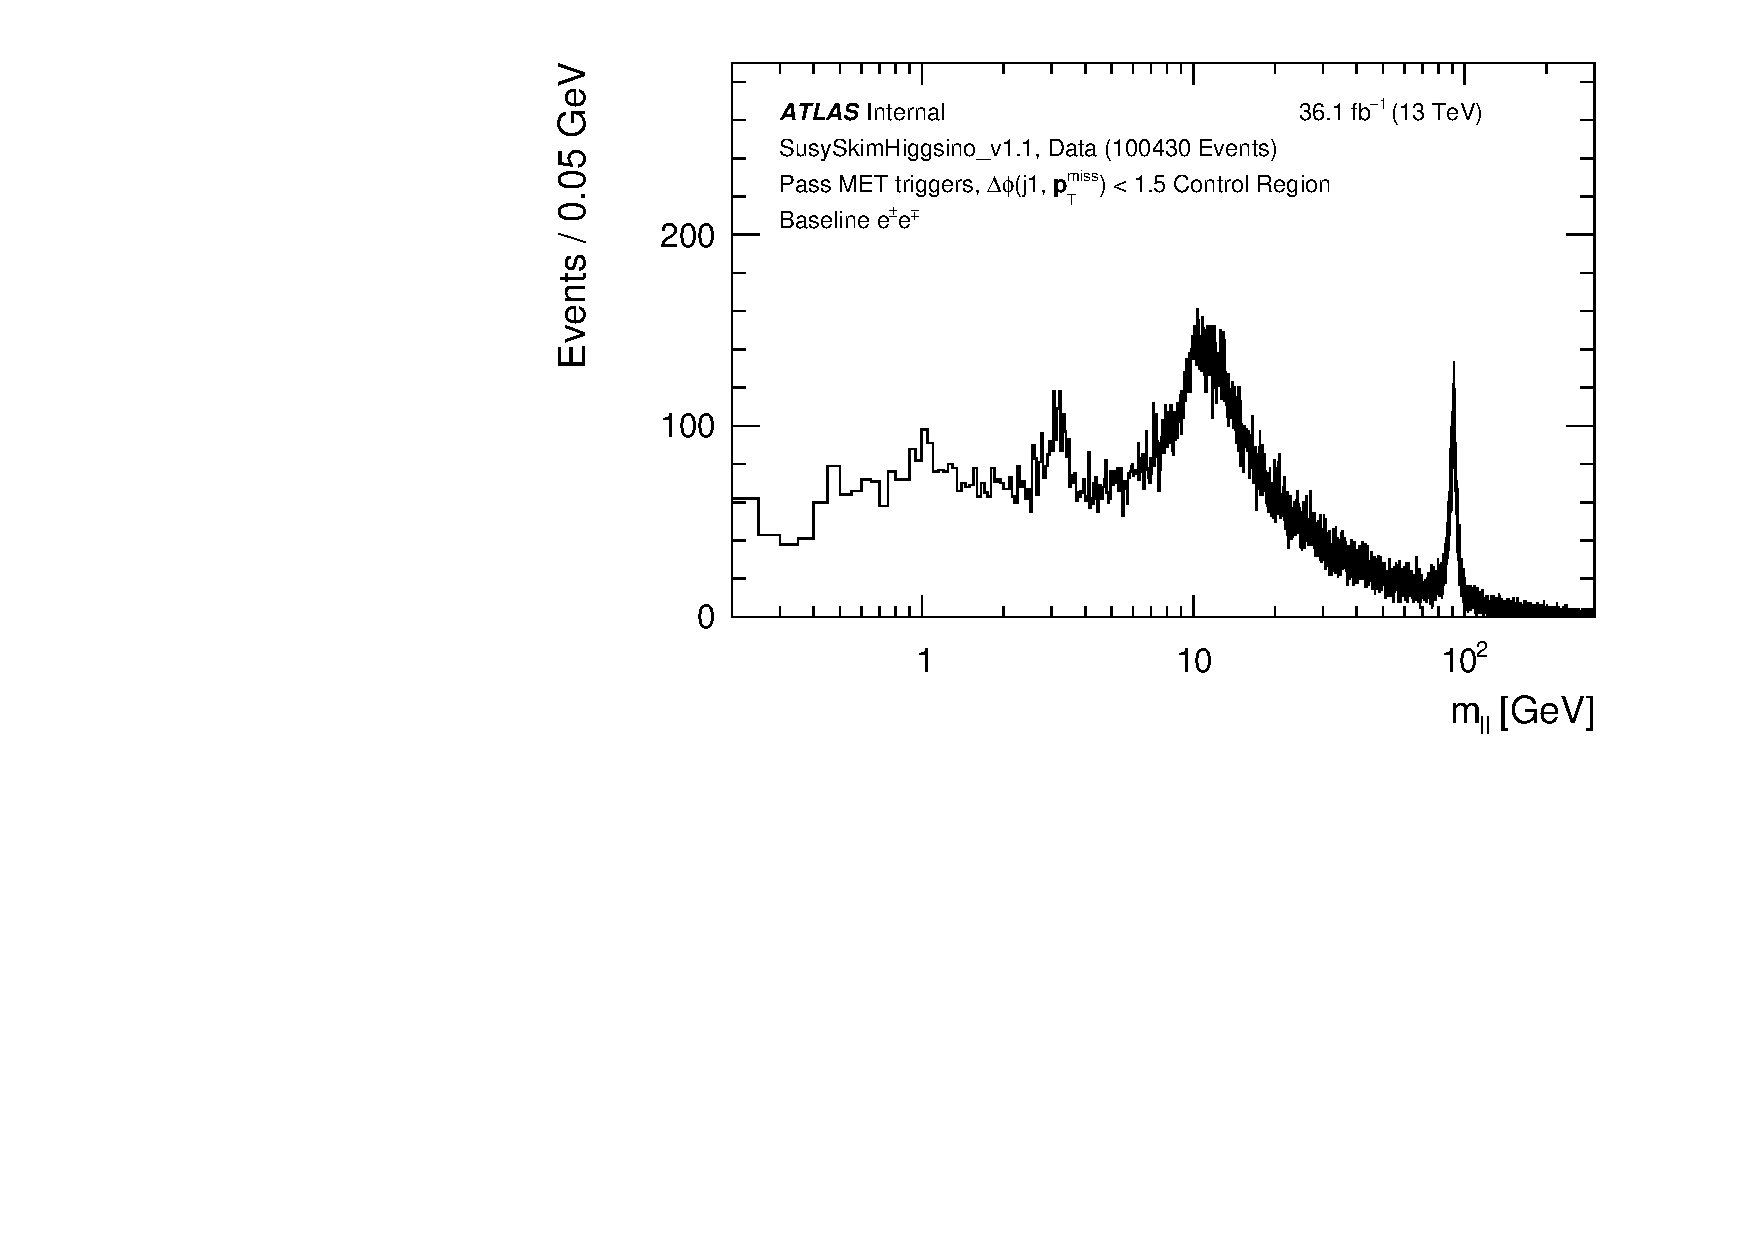
\includegraphics[scale=0.35]{dataCR_mll_ElEl_pre.pdf}
            \caption{$ee$ invariant mass}
            \label{fig:bkg_ee_invariant_mass}
        \end{subfigure}
        \begin{subfigure}[b]{0.48\textwidth}
            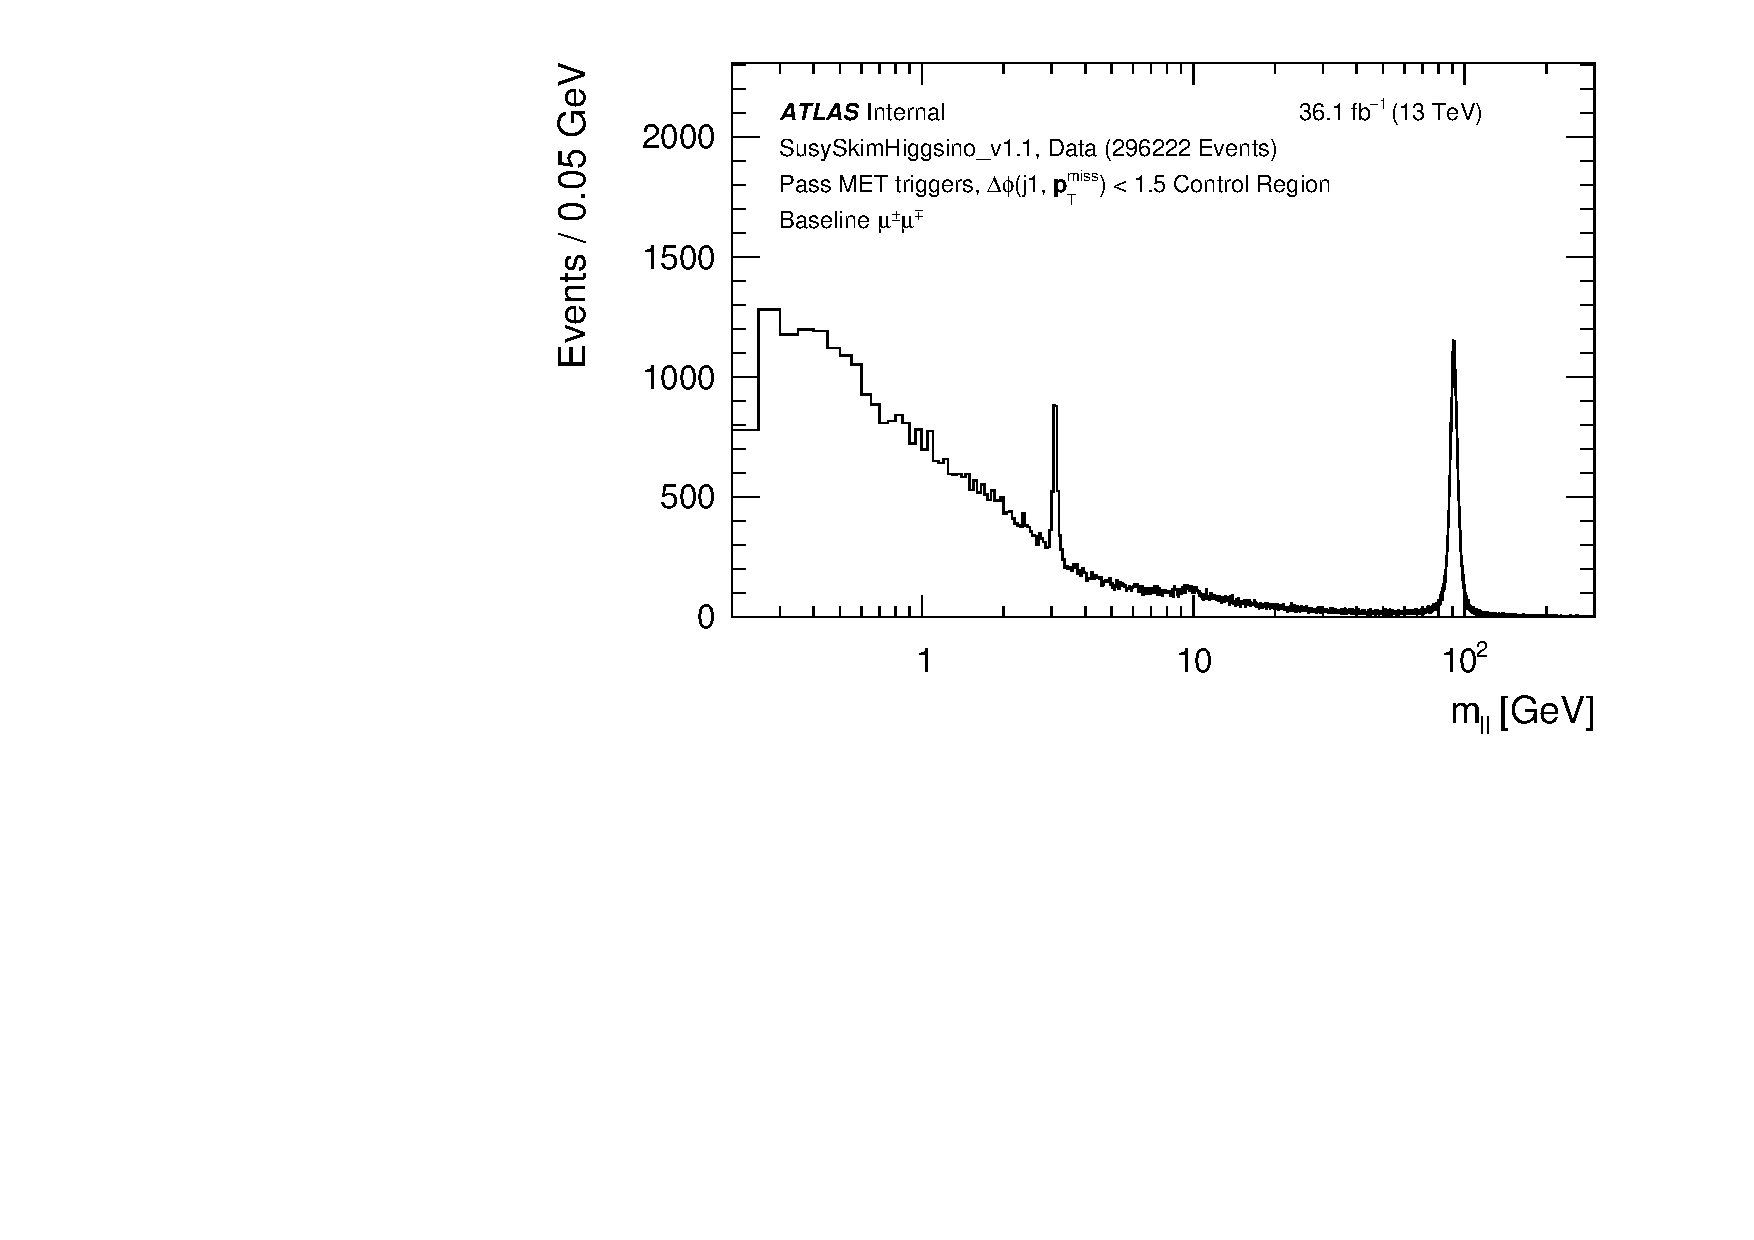
\includegraphics[scale=0.35]{dataCR_mll_MuMu_pre.pdf}
            \caption{$\mu \mu$ invariant mass}
            \label{fig:bkg_mumu_invariant_mass}
        \end{subfigure}
        \caption{The opposite sign baseline dilepton mass $m_{\ell \ell}$ spectrum.
        All data events are required to pass \met trigger and satisfies $|\Delta \phi(j_{1}, \mathbf{p}_\mathrm{T}^\mathrm{miss})| < 1.5$ requirement.
        A low mass $J/\psi$ peak can be seen in $ee$ and $\mu \mu$ invariant mass.}
        \label{fig:bkg_invariant_mass}
    \end{center}
\end{figure}

By vetoing $3.0 < m_{\ell \ell} < 3.2$~{\GeV}, the contributions from $J/\psi$ resonance can be removed efficiently.
By requiring min$|\Delta \phi($any jet, $\mathbf{p}^{\mathrm{miss}}_{\mathrm{T}})| > 0.4$, the events contain mismeasured jet causing large \met can be suppressed.
After applying these requirements, the instrumental \met background are found to be negligible.

A validation region VR-SS, which has the similar kinematic as the SR, is constructed by requiring same sign leptons in the events.
This VR is fake/non-prompt lepton enriched and can be used as a cross-checked of the fake prediction. 
Typically, the leading lepton is the real lepton and the subleading lepton is the fake/non-prompt lepton.
By considering the rate of the anti-ID leptons in data, the probability of both leptons are fake/non-prompt is found very small.
Therefore, the VR-SS are devided into $ee+\mu e$ and $\mu \mu + e\mu$ final states where the left lepton and right lepton in the pair denote the leading and subleading leptons, respectively.
The electroweakino signal contamination in VR-SS is very small and can be negelected.
Figure~\ref{fig:bkg_fake_distributions} shows the data and fake/non-prompt leptons \met distributions for $ee+\mu e$ and $\mu \mu + e\mu$ final states in the VR-SS.

\begin{figure}[ht]
    \begin{center}
        \begin{subfigure}[b]{0.48\textwidth}
            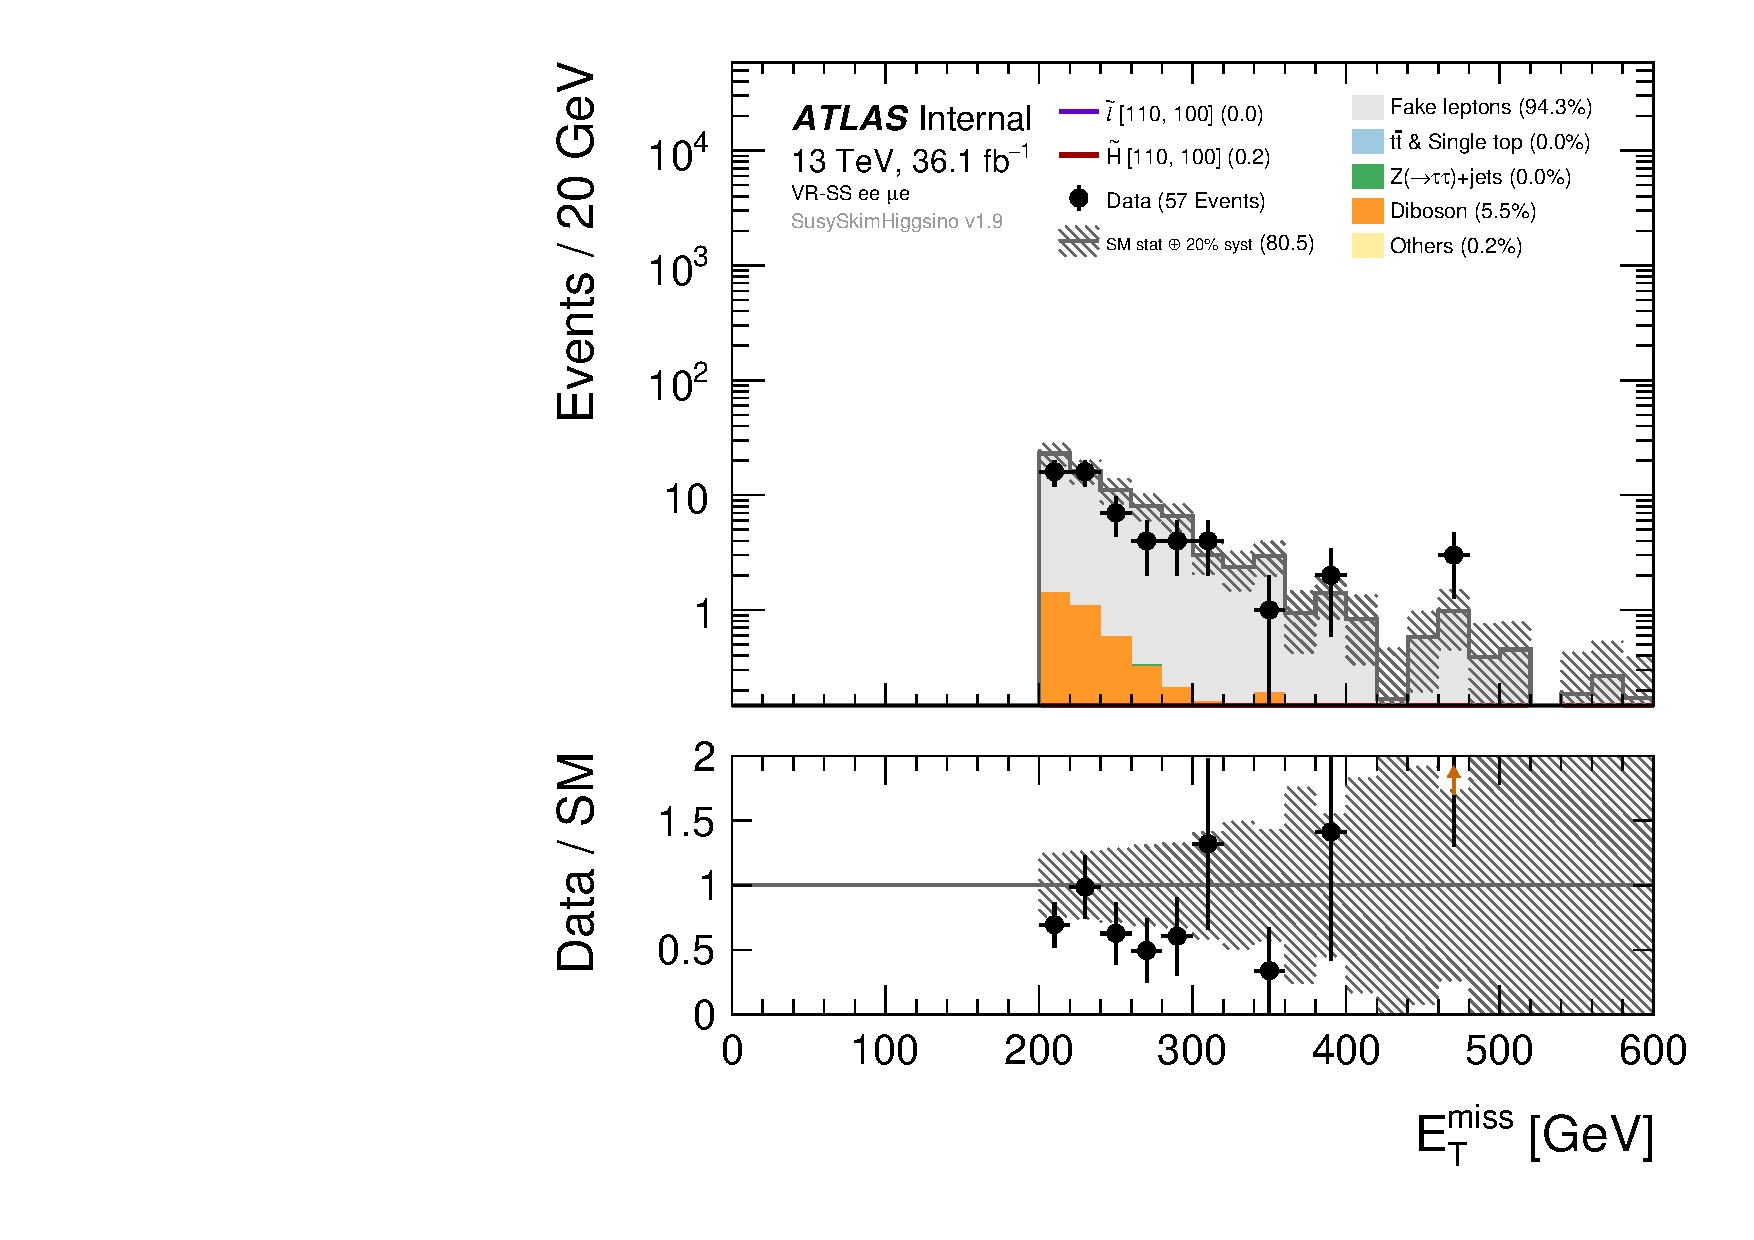
\includegraphics[scale=0.35]{hist1d_met_Et_VR-SS-ee-me.pdf}
            \caption{$ee+\mu e$}
            \label{fig:bkg_ee_mue_fake_distribution}
        \end{subfigure}
        \begin{subfigure}[b]{0.48\textwidth}
            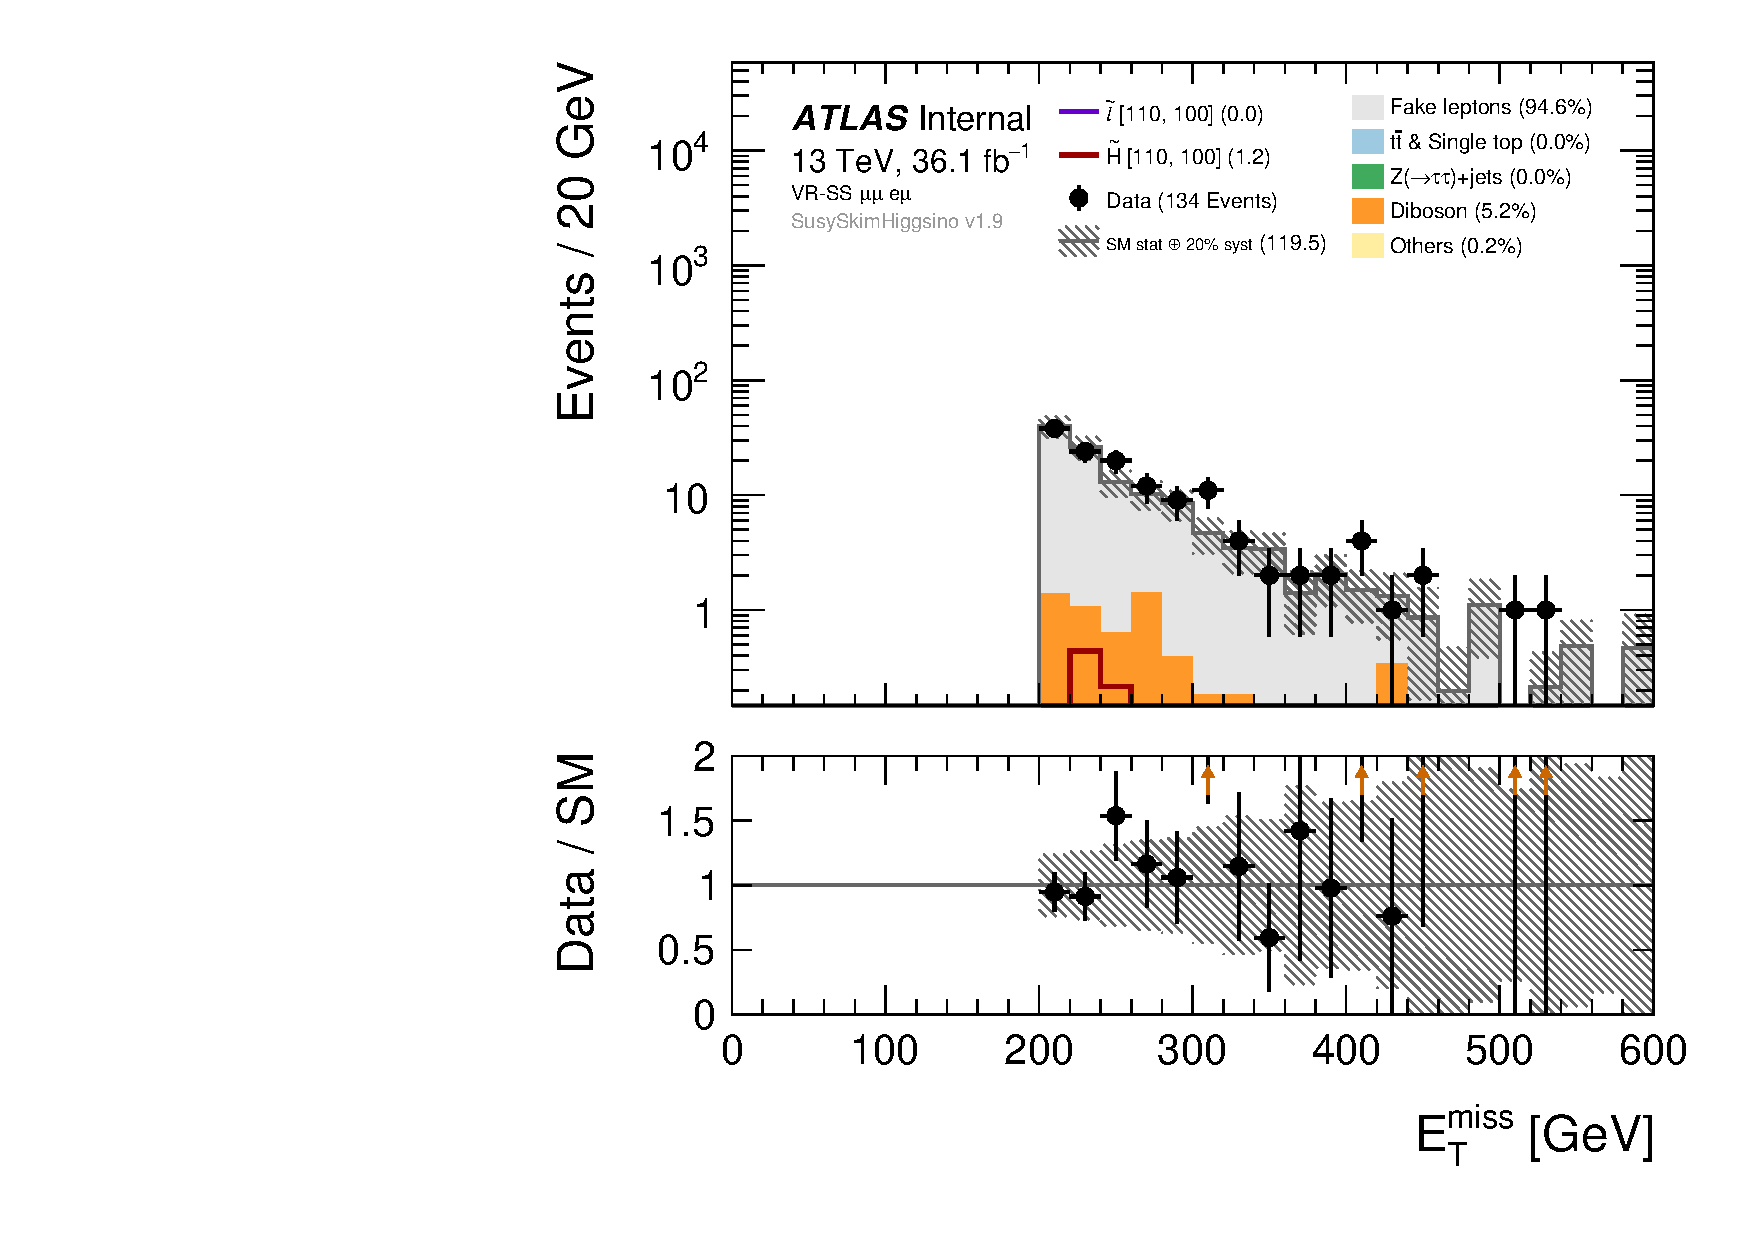
\includegraphics[scale=0.35]{hist1d_met_Et_VR-SS-mm-em.pdf}
            \caption{$\mu \mu + e\mu$}
            \label{fig:bkg_mumu_emu_fake_distribution}
        \end{subfigure}
        \caption{The data and fake/non-prompt leptons \met distributions in the VR-SS.}
        \label{fig:bkg_fake_distributions}
    \end{center}
\end{figure}

%%%
%%%
%%%

\section{Systematic uncertainties}
\label{sec:bkg_systematic_uncertainties}
The systematic uncertainty includes the uncertainties due to theoretical modeling and experiment sources.
The theoretical uncertainty arises from the MC simulation such as cross-section calculation, the parton distribution function (PDF), and renormalization and factorization scales.
The experimental uncertainty arises from the object reconstruction, pileup measurement, and estimation using data-driven method.

%%%
%%%
%%%

\subsection{Theoretical uncertainty}
\label{subsec:bkg_theoretical_uncertainty}

%%%
%%%
%%%

\subsubsection{SUSY signal uncertainty}
\label{subsubsec:bkg_susy_signal_uncertainty}
The theoretical uncertainty in the SUSY signal is measured by varying the renormalization, factorization parameters and CKKW-L matching scales in the MG5\_{\scriptsize A}MC@NLO
generator and the shower tune parameters in the {\PYTHIA}.
The uncertainties are found to range from 20\% to 40\% in the signal acceptance depending on the mass splitting of the SUSY particles and the production process.
The uncertainties due to PDF uncertainties are studied and amount to 15\% at most for large $\widetilde{\chi}^{0}_{2}$ mass.

%%%
%%%
%%%

\subsubsection{SM background uncertainty}
\label{subsubsec:bkg_sm_bkg_uncertainty}
There are three major factors affect the dominant SM backgrounds \ttbar, $tW$, $Z^{(*)}/\gamma^{*}(\to \tau \tau)$+jets, and diboson process.
The envelop is assigned to the theoretical uncertainty.
The uncertainties due to the QCD renormalization and factorization scales are evaluted by varying the generator parameters up and down by a factor of 2.
The uncertainties due to the sctrong coupling constant $\alpha_{S}$ are evaluted by varying the $\alpha_{S}$.
The impact on the acceptance is assigned to the theoretical uncertainty.
The uncertainties due to the PDF are evaluted by PDF sets \texttt{CT14}, \texttt{MMHT2014}, and \texttt{NNPDF}.
The variations in acceptance are summarized and the envelope is assigned to the theoretical uncertainty.
Events with all lepton flavors are used and the uncertainties are evaluted in all SRs and CRs.
The final uncertainty is evaluted by adding all components in quadrature.

%%%
%%%
%%%

\subsection{Experimental uncertainty}
\label{subsec:bkg_experimental_uncertainty}

%%%
%%%
%%%

\subsubsection{Combined performance uncertainty}
\label{subsubsec:bkg_combined_performance uncertainty}
The uncertainties of lepton reconstruction, identification, and isolation as well as the uncertainties of energy and momentum scale and resolution are considered, but they are found to be small.
The pileup in the MC samples is not the same as the one observed in data.
The $\langle \mu \rangle$ profile is the average number of interactions per bunch crossing and the $\langle \mu \rangle$ in data is scaled by 1/1.16 to obtain a better data/MC agreement.
The uncertainty of the pileup reweighting is obtained by varying the scaling factor between 1.00 and 1.23.
The uncertainties from the jet energy scale (JES) and resolution (JER) are considered.
Five up and down variations are used to obtain JES uncertainty and a up variation is used to obtain JER uncertainty.
Finally, the luminosity uncertainty is 3.2\% for 2015+2016 combined datasets.

%%%
%%%
%%%

\subsubsection{Fake factor uncertainty}
\label{subsubsec:bkg_fake_factor_uncertainty}
The major experimental uncertainty is the fake/non-prompt lepton prediction from the fake factor method.
The fake factor uncertainty arises from the sample size used to measure the fake factors, the prompt lepton contamination in anti-ID region, the kinematic between the measurement region and the SRs, and the differences between the fake factor estimation and observed data in the VR-SS.

Figure~\ref{fig:bkg_relative_systematic_uncertainties} shpws the relative size of various uncertainties in the background predictions in the exclusive electroweakino SRs.
The fake factor uncertainty is shown separatively from the other experimental uncertainties due to the relatively large contribution.

\begin{figure}[htbp]
    \begin{center}
        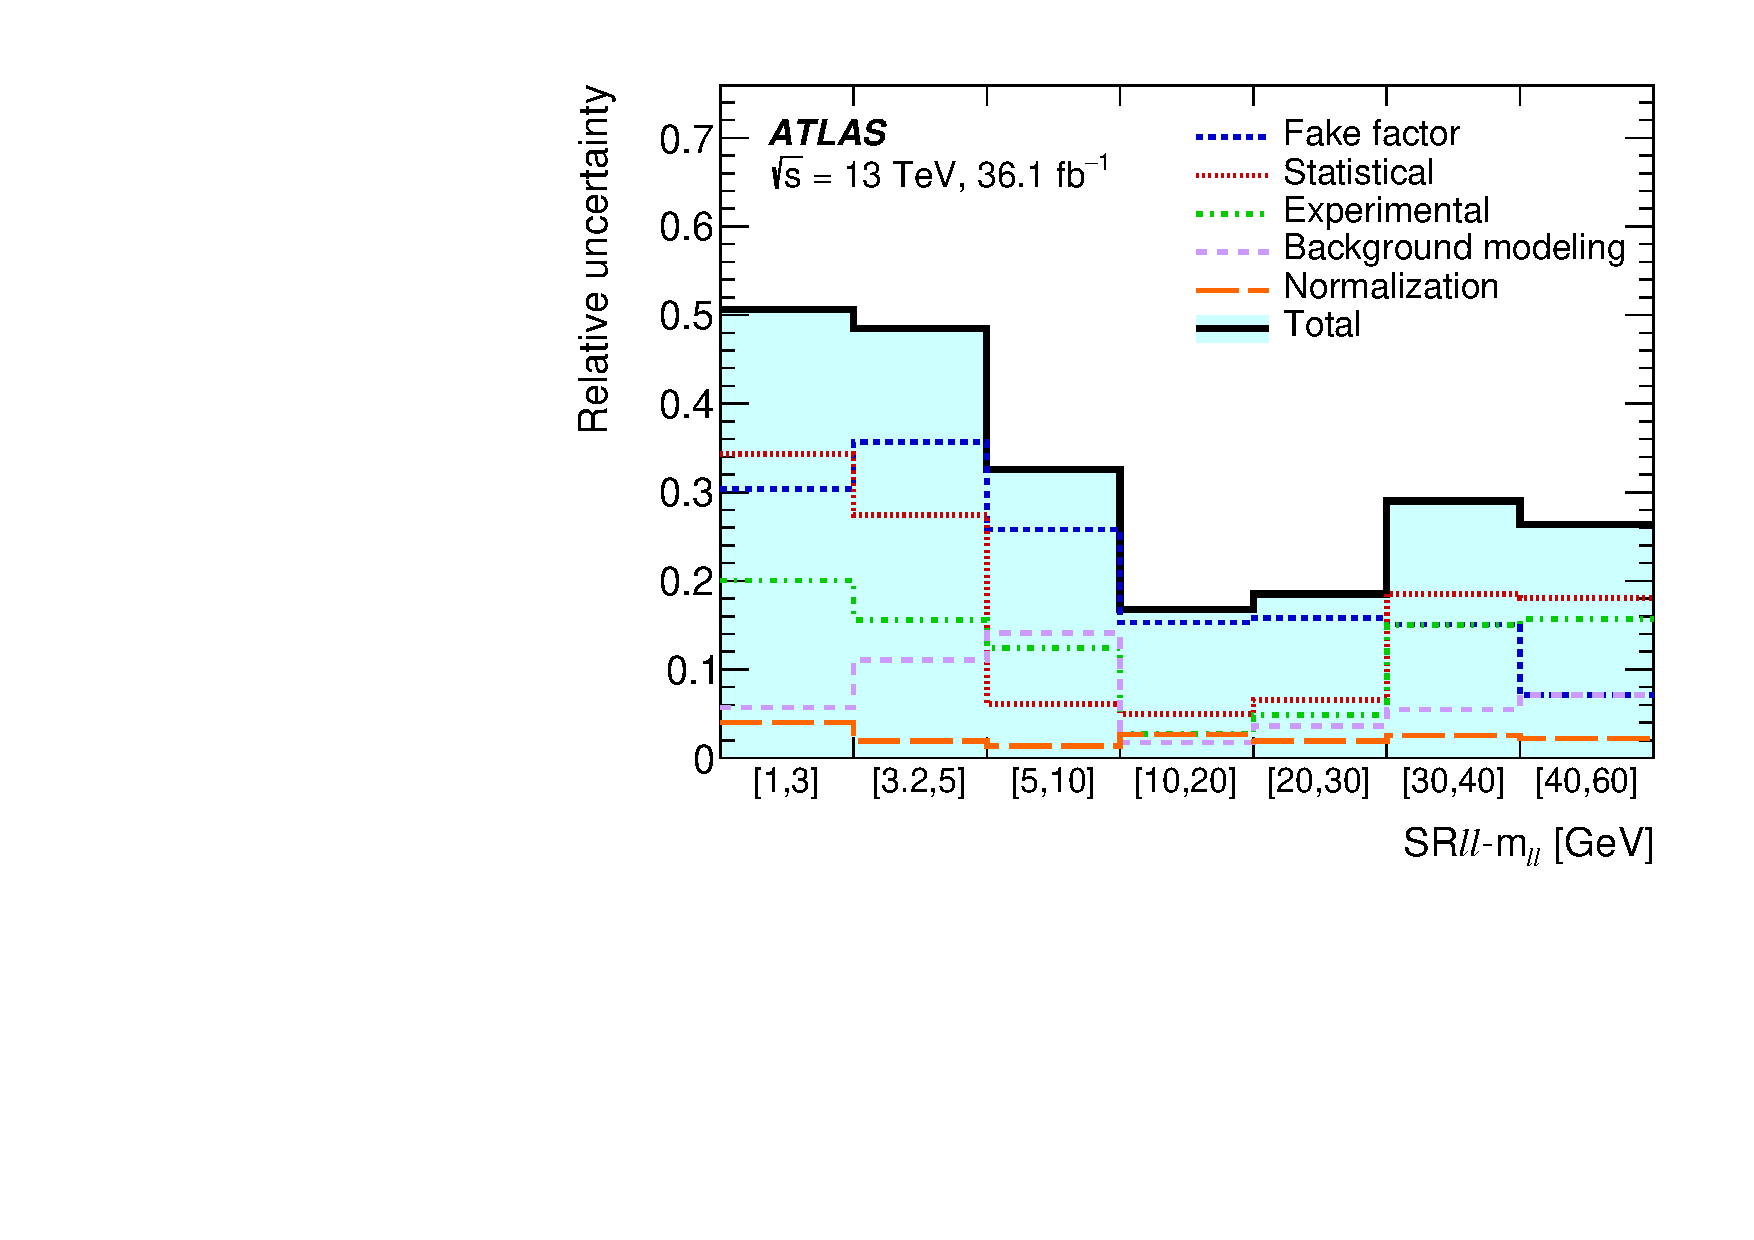
\includegraphics[scale=0.4]{fig_05a.pdf}
        \caption{The relative systematic uncertainties in the background prediction in the exclusive electroweakino SRs.}
        \label{fig:bkg_relative_systematic_uncertainties}
    \end{center}
\end{figure}
